\chapter{基于采样的近似推断}
\label{chap:pgm-sampling}

第~\ref{chap:pgm-elimination}、\ref{chap:pgm-junction-tree}章的精确推断和第~\ref{chap:pgm-variational}章的变分近似，都用确定的数值或近似分布描述后验。采样推断不直接求出整个后验分布，而是从后验中抽取一批代表性随机样本：估计故障的后验概率时，统计样本中故障出现的比例；估计期望时，对样本上的函数值取平均。当中间因子过大、高维积分没有闭式解，或合适的变分分布族难以选定时，样本统计量通常较少依赖模型的具体解析形式。它的代价是答案带随机误差且通常只能近似；增加样本可以压低误差，同一批样本还能回答多个查询。

从后验采样通常并不比求后验更容易，因为实际往往只知道未归一化的联合权重$p(\bm{x},\bm{z})$，不知道归一化常数。本章讨论四种间接获得后验代表性样本的机制及其成立条件。直接从目标生成独立样本时，可用大数定律分析样本均值；目标难以直接采样时，重要性采样从提议分布生成候选，再用权重修正差异；高维下难以构造全局提议时，MCMC从当前状态作局部移动，靠满足条件的Markov链使长期访问比例逼近后验；观测随时间逐步到来时，序贯蒙特卡洛/粒子滤波递推样本与权重，并淘汰低质量样本。每种机制分别讨论估计量的极限条件、有限计算误差和诊断方法。

\section{采样推断的定义}
\label{sec:pgm-sampling-definition}

采样估计建立在一个共同事实上：如果存在一批独立且服从后验的样本，就可以用样本平均代替后验期望，并量化估计误差。后续各种采样器主要解决如何获得这样的样本。先设观测为$\bm{x}$，潜变量为$\bm{z}$，固定模型参数并省略其记号。把目标后验写为
\begin{equation}
  \begin{aligned}
    p(\bm{z}\mid\bm{x})&=\frac{\gamma(\bm{z})}{Z_{\bm{x}}},&
    \gamma(\bm{z})&=p(\bm{x},\bm{z}),\\
    Z_{\bm{x}}&=\int\gamma(\bm{z})\,\mathrm{d}\bm{z},&
    I_h&=\mathbb{E}_{p(\bm{z}\mid\bm{x})}[h(\bm{z})].
  \end{aligned}
  \label{eq:pgm-sampling-target}
\end{equation}
其中$0<Z_{\bm{x}}<\infty$，$h$是待求期望的实值函数。本章的积分也涵盖离散情形，此时改为求和，$p$表示概率质量而非密度。$\gamma$可以计算到一个与$\bm{z}$无关的正比例常数；这足以计算后验期望，却不足以确定原模型的证据$Z_{\bm{x}}$。估计证据时，必须知道$\gamma$的实际尺度。

若能直接从后验获得独立同分布的$\bm{z}_1,\ldots,\bm{z}_n$，就可以用函数值的样本均值估计$I_h$：
\begin{equation}
  \widehat I_{h,n}=\frac{1}{n}\sum_{i=1}^{n}h(\bm{z}_i).
  \label{eq:pgm-sampling-direct-estimator}
\end{equation}
选择$h(\bm{z})=\mathbb{I}\{\bm{z}\in B\}$，即事件$B$发生时取$1$、否则取$0$的指示函数，就得到后验事件概率的估计；选择某个分量或分量乘积，则得到均值或二阶矩。同一批样本可以用于多个查询，各查询的误差由相应的函数$h$决定。采样平均、方差缩减和Markov链长期平均的概率基础可参考\BookChapterRef{chap:random-sequences-and-processes}{卷2《数学准备：概率、因果与决策》的“随机序列与随机过程”章}。

独立样本的极限理论提供这一估计量的正确性依据。可积$h$使样本均值几乎必然收敛；方差$\sigma_h^2=\operatorname{Var}_p(h)$有限时，估计量还满足下列方差与极限关系：
\begin{equation}
  \begin{aligned}
    \mathbb{E}[\widehat I_{h,n}]&=I_h,&
    \operatorname{Var}(\widehat I_{h,n})&=\frac{\sigma_h^2}{n},\\
    \sqrt n(\widehat I_{h,n}-I_h)&\xrightarrow{\mathrm{d}}
      \mathcal{N}(0,\sigma_h^2).
  \end{aligned}
  \label{eq:pgm-sampling-iid-clt}
\end{equation}
\term{蒙特卡洛标准误}（Monte Carlo standard error, MCSE）衡量重复运行估计过程时答案的波动，即再独立抽取同样多的一批样本时平均答案的变动幅度。独立样本下可用$s_h/\sqrt n$估计，其中$s_h^2$是$h(\bm z_i)$的样本方差。它与后验标准差有明确区别：后者描述模型本身固有的不确定性（故障是否可能发生），不随样本增多而消失；MCSE描述有限采样带来的计算波动（对该概率估计的偏差程度），随$n$增大趋于零。


\begin{example}[报警后的故障概率]
  \label{ex:pgm-sampling-device}
  沿用人工构造的设备模型$F\to H\to A\leftarrow S$：$F$表示故障，$H$表示过热，$A$表示报警，$S$表示传感器失灵。根节点$F,S$独立，且
  \[
    \begin{aligned}
      p(F=1)&=0.1,&p(S=1)&=0.05,\\
      p(H=1\mid F=1)&=0.8,&
      p(H=1\mid F=0)&=0.1.
    \end{aligned}
  \]
  报警条件表仍与前面的精确推断相同：
  \[
    \begin{array}{ccccc}
      (h,s)&(0,0)&(1,0)&(0,1)&(1,1)\\
      p(A=1\mid h,s)&0.01&0.9&0.7&0.99
    \end{array}
  \]
  边缘化故障得到$p(H=1)=0.17$，从而
  \[
    \begin{aligned}
      p(A=1\mid H=0)&=0.95\times0.01+0.05\times0.7=0.0445,\\
      p(A=1\mid H=1)&=0.95\times0.9+0.05\times0.99=0.9045,\\
      p(A=1)&=0.83\times0.0445+0.17\times0.9045=0.1907,\\
      p(F=1,A=1)&=0.1(0.2\times0.0445+0.8\times0.9045)=0.07325.
    \end{aligned}
  \]
  因此精确答案为$p(F=1\mid A=1)=0.07325/0.1907\approx0.384111$。若能够取得$10000$个独立后验样本，故障比例的理论标准误约为$\sqrt{0.384111(1-0.384111)/10000}=0.004864$。这个小模型的精确答案用于校验采样计算，不是实际设备数据。
\end{example}

改变样本生成机制后，误差分析也要随之改变。重要性样本由提议生成，估计方差取决于加权函数；一条Markov链上的状态通常相关，样本均值的方差需要计入协方差；重采样粒子还可能共享祖先。后文分别建立这些机制下的正确性条件，再分析相应的计算误差。普通蒙特卡洛误差与方差缩减的系统论述见Owen\scite{pgm-sampling-owen2013}。

\section{独立蒙特卡洛方法}
\label{sec:pgm-sampling-independent}

这一节讲独立蒙特卡洛的三种递进办法：能直接按目标生成时直接采样；直接采样困难但能找到一个“罩住”目标的简单分布时，用拒绝采样筛选；连罩住都困难时，保留所有候选、改用连续权重修正，即重要性采样。三者每次都使用新的独立随机输入，候选彼此独立，但自归一化权重共用一个随机分母，估计量的分析还需考虑这一比值结构。

\subsection{直接采样、祖先采样与拒绝采样}
\label{sec:pgm-sampling-direct-rejection}

当目标分布本身带有容易操作的生成规则（例如有向图的局部条件分布）时，可以按变量之间的依赖顺序把一个完整样本“逐步抽出来”，无需知道难算的归一化常数。每次生成完整记录时使用新的独立随机输入，得到的记录之间才具有独立性。

在有向无环图上，\term{祖先采样}（ancestral sampling）按拓扑顺序逐个生成节点，使每个节点采样时都已知道其父节点的取值。若一次生成$\bm{x}$时，第$i$个节点使用$p(x_i\mid\bm{x}_{\operatorname{pa}(i)})$，则整次生成的概率恰为这些条件概率之积，也就是图模型的联合分布。样本内部的各节点通常不独立，独立的是从头运行得到的不同完整样本。一次生成的成本包括拓扑遍历和所有局部条件分布的采样成本；后者取决于各条件分布的实现。

祖先采样很容易抽到联合分布，但我们真正想要的是给定证据（如$A=1$）后的后验。一个朴素办法是：照常按先验抽完整样本，然后只保留恰好符合证据的样本、丢弃其余。在设备模型上，若按先验生成$F,S,H$后直接把$A$强行设为$1$，保留下来的故障比例仍是先验的$0.1$，并不是后验；只有连同$A$一起按模型生成、再仅保留$A=1$的样本，所保留记录才服从后验，故障概率为$0.384111$。这种“先从简单分布生成候选、再按某个规则决定去留”的做法就是\term{拒绝采样}（rejection sampling）的特例。

拒绝采样的一般设定是：找一个容易采样的提议分布$q$，并让它的密度在每一处都不低于目标密度（允许差一个常数倍），候选落在目标密度相对越高的位置就越可能被接受、越低则越可能被拒绝。设$q(\bm{z})$为提议密度，已知常数$c<\infty$使$\gamma(\bm{z})\leq c q(\bm{z})$在整个目标支撑集上成立。独立生成$\bm{z}\sim q$和$u\sim\operatorname{Uniform}(0,1)$，当$u\leq\gamma(\bm{z})/[c q(\bm{z})]$时接受。对任意可测集合$B$，
\begin{equation}
  \begin{aligned}
    \mathbb{P}(\bm{z}\in B,\text{接受})
      &=\int_B q(\bm{z})\frac{\gamma(\bm{z})}{c q(\bm{z})}
        \,\mathrm{d}\bm{z}
        =\frac{1}{c}\int_B\gamma(\bm{z})\,\mathrm{d}\bm{z},\\
    \mathbb{P}(\text{接受})&=\frac{Z_{\bm{x}}}{c}.
  \end{aligned}
  \label{eq:pgm-sampling-rejection}
\end{equation}
相除便得到$\mathbb{P}(\bm{z}\in B\mid\text{接受})=\int_B p(\bm{z}\mid\bm{x})\,\mathrm{d}\bm{z}$。因此按固定规则独立重复试验，直到得到指定数量的接受样本，会产生独立同分布的目标样本。每个接受样本平均需要$c/Z_{\bm{x}}$次提议。这一结论依赖全局包络条件。只检查已生成的位置，无法保证未访问区域也满足相同的接受规则。

在报警例子中，匹配证据的接受率为$0.1907$，平均约$5.244$次联合采样得到一个后验样本。若有多个稀有离散证据，联合匹配概率可能很小；连续证据的精确等值事件通常概率为零，需要使用密度条件化等其他采样构造。高维包络也容易变松：若归一化目标和提议分别按坐标分解，每维包络常数为$m>1$，乘积包络的接受率便是$m^{-d}$。后验越集中而提议越分散，越多计算会用在最终丢弃的候选上。

\subsection{重要性采样}
\label{sec:pgm-sampling-importance}

拒绝采样的最大问题是大量候选会被白白丢弃，尤其当证据稀有、维度很高时接受率极低。换个角度：与其把不太符合目标的候选直接扔掉，不如全都保留，但让每个候选对最终估计的“话语权”按它与目标的吻合程度加权——吻合得好的权重大、吻合得差的权重小。\term{重要性采样}（importance sampling, IS）正是这样做的：从易采样的$q$生成候选，并以目标与提议的密度比修正抽样频率。这要求$p\ll q$，即$q$必须覆盖目标的所有正概率区域（否则目标在那些区域的质量永远采不到、也无从修正）；连续情形按测度理解，零测集上的密度取值不影响结论。

如果目标密度已归一化，令$r(\bm{z})=p(\bm{z}\mid\bm{x})/q(\bm{z})$，便有
\begin{equation}
  \begin{aligned}
    I_h&=\int h(\bm{z})r(\bm{z})q(\bm{z})\,\mathrm{d}\bm{z},\\
    \widehat I_{h,n}^{\mathrm{IS}}
      &=\frac{1}{n}\sum_{i=1}^{n}r(\bm{z}_i)h(\bm{z}_i).
  \end{aligned}
  \label{eq:pgm-sampling-is}
\end{equation}
只要$\mathbb{E}_p|h|<\infty$，这个估计无偏且一致；有限方差还要求$\mathbb{E}_q[r^2h^2]<\infty$。目标区域若只被$q$赋予很小概率，偶尔出现的巨大权重会主导结果。支持覆盖保证目标区域有机会被提议访问，加权矩条件进一步控制罕见访问带来的波动。

图模型往往只提供$\gamma$。令$w_i=\gamma(\bm{z}_i)/q(\bm{z}_i)$，同时估计分子积分和归一化常数，得到\term{自归一化重要性采样}（self-normalized importance sampling, SNIS）：
\begin{equation}
  \begin{aligned}
    \widehat Z_{\bm{x}}&=\frac{1}{n}\sum_{i=1}^{n}w_i,&
    \bar w_i&=\frac{w_i}{\sum_{j=1}^{n}w_j},\\
    \widehat I_{h,n}^{\mathrm{SNIS}}
      &=\frac{\frac{1}{n}\sum_i w_i h(\bm{z}_i)}
              {\frac{1}{n}\sum_i w_i}
       =\sum_i\bar w_i h(\bm{z}_i).
  \end{aligned}
  \label{eq:pgm-sampling-snis}
\end{equation}
要求本次权重和非零。$\widehat Z_{\bm{x}}$无偏，但两个无偏估计的比值通常有偏，因为随机分母不能移到期望之外。在支撑集覆盖、$0<\mathbb{E}_q w=Z_{\bm{x}}<\infty$和$\mathbb{E}_q|wh|<\infty$时，分子、分母分别由大数定律收敛，故比值仍然一致。因此，比值的有限样本偏差与样本数增长后的渐近一致性可以同时成立。

设备例子可以令$q(f,h,s)=p(f)p(s)p(h\mid f)$，不抽取已知的$A$，而令$w(f,h,s)=p(A=1\mid h,s)$。这称为\term{似然加权}（likelihood weighting）：证据通过似然而非硬性筛选影响候选。图~\ref{fig:pgm-sampling-importance}比较先验与报警后的$(H,S)$分布。先验最常生成“既不过热也未失灵”，但这一状态很难解释报警；乘上似然以后，它只占约$4.13\%$的后验质量。

\begin{figure}[!t]
  \centering
  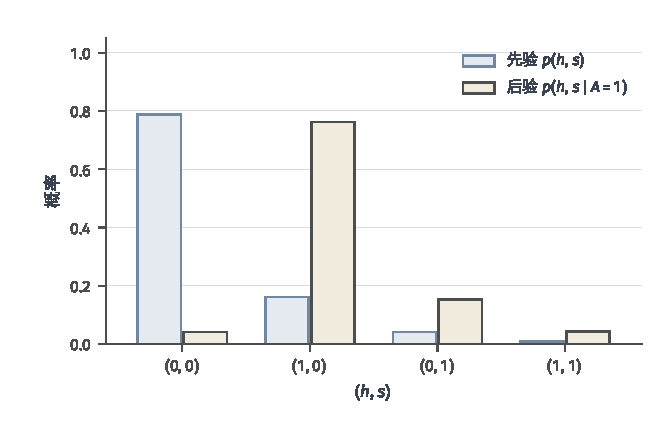
\includegraphics[width=105.412mm]{figures/06-probabilistic-graphical-models/02-inference/matplotlib/pgm-sampling-importance/figure.pdf}
  \caption{人工设备模型中$(H,S)$的先验与给定$A=1$后的后验。横轴每组的两位数依次为$h,s$；淡蓝柱表示先验，淡黄色柱表示后验。权重改变已有候选的贡献；未被抽到的类别仍需依靠后续生成访问。}
  \label{fig:pgm-sampling-importance}
\end{figure}

表~\ref{tab:pgm-sampling-weight-example}用四个可能的独立先验样本展示似然加权。直接计数的故障比例为$1/4$，加权比例为$0.9/(0.01+0.9+0.9+0.7)\approx0.358566$。权重按目标修正了候选贡献，但四次抽样仍有明显的有限样本波动，所得比例与精确后验不同。

\begin{table}[!t]
  \centering
  \begin{tabular}{ccccc}
    \toprule
    样本$i$ & $(f_i,h_i,s_i)$ & $w_i$ & $\mathbb{I}\{f_i=1\}$ & $w_i\mathbb{I}\{f_i=1\}$\\
    \midrule
    1 & $(0,0,0)$ & $0.01$ & $0$ & $0$\\
    2 & $(1,1,0)$ & $0.90$ & $1$ & $0.90$\\
    3 & $(0,1,0)$ & $0.90$ & $0$ & $0$\\
    4 & $(0,0,1)$ & $0.70$ & $0$ & $0$\\
    \bottomrule
  \end{tabular}
  \caption{似然加权的四样本教学计算。分母是全部权重之和，分子仅累加故障样本的权重。}
  \label{tab:pgm-sampling-weight-example}
\end{table}

提议的尾部决定极端权重出现的频率。即使提议很好地匹配后验峰附近，尾部事件估计仍需要足够的尾部覆盖。以一维标准正态目标$p=\mathcal{N}(0,1)$和$q=\mathcal{N}(0,s^2)$为例，其中$s>0$。二者的支撑集相同，但这只保证每个目标区域都有机会被访问。要判断权重的波动是否具有有限二阶矩，需要计算
\[
  \mathbb{E}_q[r^2]
    =\int \left(\frac{p(z)}{q(z)}\right)^2q(z)\,\mathrm{d}z
    =\int\frac{p(z)^2}{q(z)}\,\mathrm{d}z.
\]
将两个高斯密度代入，被积函数除去与$z$无关的正常数以后为
\[
  \frac{p(z)^2}{q(z)}
    \ \propto\ \exp\left[\left(-1+\frac{1}{2s^2}\right)z^2\right].
\]
当二次项系数$-1+1/(2s^2)$为负时，被积函数在两端都按高斯速度衰减，积分有限。系数为零时，被积函数是正常数，在整条实线上积分仍然发散；系数为正时，它随$|z|$增长，积分也发散。因此$\mathbb{E}_q r^2$只有在$s^2>1/2$时才有限。这是权重本身的二阶矩判据；具体查询的IS方差还要检查前述$\mathbb{E}_q[r^2h^2]$，不能仅凭权重二阶矩替任意$h$作保证。

提议过窄时，算法可以满足一致性的条件，却没有通常所需的有限权重二阶矩；重复运行中偶发的大权重会破坏熟悉的误差估计。如何构造尾部足够宽、同时不过度浪费样本的提议，是重要性采样的主要计算问题；相关分析可参见Owen教材的第9章\scite{pgm-sampling-owen2013}

\subsection{方差缩减}
\label{sec:pgm-sampling-variance-reduction}

增加样本数$n$总能压低误差，但代价是采更多样本。蒙特卡洛里还有另一类不增加样本、而是巧妙利用解析计算来减小单次随机贡献波动的办法，统称为方差缩减。这里介绍两种最常用的：一种用一个期望已知的相关量去抵消共同波动（控制变量），另一种把原本要靠抽样的部分改用精确积分算掉（Rao–Blackwell化）。

除了增加独立样本数，还可以通过减小单次随机贡献的方差来降低MCSE。设一次独立抽样原本给出随机贡献$Y$，待求量为$\mathbb{E}Y$。若能同时计算另一个随机量$G$，且其期望$\mu_G$已知，就可以用$G-\mu_G$记录这次抽样相对已知均值的偏离。对预先固定的系数$a$，以$Y-a(G-\mu_G)$替换$Y$不会改变期望，因为被减去部分的期望为零。这就是控制变量（control variates）的作用：利用已知期望修正样本函数。在$Y,G$均有有限方差时，
\[
  \operatorname{Var}\bigl(Y-a(G-\mu_G)\bigr)
    =\operatorname{Var}(Y)-2a\operatorname{Cov}(Y,G)
       +a^2\operatorname{Var}(G).
\]
若$\operatorname{Var}(G)>0$，使该二次式最小的系数为
\[
  a=\frac{\operatorname{Cov}(Y,G)}{\operatorname{Var}(G)}.
\]
代入这个系数后，方差的减少量为$\operatorname{Cov}(Y,G)^2/\operatorname{Var}(G)$。因此收益来自两种贡献之间可被抵消的共同波动，并非任意选择控制变量和系数都会减小方差。若总体协方差未知，可以用独立的先导样本估计$a$，再在正式抽样中固定该系数；若用同一批样本估计$a$并回代，系数与样本贡献会相互依赖，需另查偏差，不能直接继承固定系数时的无偏结论。

另一种波动来自完整记录中并非必须抽取的变量。若保留随机量$U$以后，仍能解析计算其余随机性下的条件平均，就可以把$Y$替换为$\widetilde Y=\mathbb{E}[Y\mid U]$。这种Rao--Blackwell化（Rao--Blackwellization）将部分抽样替换为条件积分。在图模型中，局部消元可以解析消去部分节点，仅对保留变量采样。条件积分必须使用原联合分布在给定$U$后的条件分布；这样的相容条件期望才保持原均值。由迭代期望和全方差关系，有限二阶矩下有
\[
  \begin{aligned}
    \mathbb{E}\widetilde Y&=\mathbb{E}Y,\\
    \operatorname{Var}(Y)
      &=\operatorname{Var}(\widetilde Y)
        +\mathbb{E}\bigl[\operatorname{Var}(Y\mid U)\bigr]
       \geq\operatorname{Var}(\widetilde Y).
  \end{aligned}
\]
被消去的是给定$U$以后仍会发生的抽样波动，右侧的条件方差项正好度量这部分波动。在相同独立抽样次数下，样本均值的方差也随之不增。

若目标是设备的先验报警概率，可以抽取完整$(F,H,S,A)$并平均$\mathbb{I}\{A=1\}$，也可以只抽取$F$，把其余节点解析消去。这里原贡献是$Y=\mathbb{I}\{A=1\}$，保留变量是$U=F$，所以替换后的贡献为$\mathbb{E}[Y\mid F]=p(A=1\mid F)$。它按原模型的$p(H,S,A\mid F)$积分，而非另换一个容易计算的条件分布。当$F=0$时，这个条件报警概率为$0.1305$；当$F=1$时为$0.7325$。两者均值都是$0.1907$，但前者单样本方差为$0.1907(1-0.1907)=0.15433351$，后者为$0.1\times0.9(0.7325-0.1305)^2=0.03261636$。解析计算减少了相同独立抽样次数下的方差；是否节约总时间，还要比较条件积分的成本。

方差缩减需要作用于完整估计量。SNIS的分子贡献为$wh$，分母贡献为$w$，因此要按提议的条件分布同时积分这两个量，保持权重与函数的相容关系。具体地，把提议下的变量分为$(U,V)$，仅抽取$U_i\sim q_U$，再计算
\[
  \begin{aligned}
    A(U)&=\mathbb{E}_q[w(U,V)h(U,V)\mid U],\\
    B(U)&=\mathbb{E}_q[w(U,V)\mid U],\\
    \widehat I_{h,n}^{\mathrm{RB\text{-}SNIS}}
      &=\frac{\sum_{i=1}^{n}A(U_i)}{\sum_{i=1}^{n}B(U_i)}.
  \end{aligned}
\]
这两个条件平均都使用$q(V\mid U)$，所以分子与分母的期望仍分别为$Z_{\bm{x}}I_h$和$Z_{\bm{x}}$。权重和非零且原来的可积性条件成立时，比值仍然一致；它通常仍有有限样本偏差。在对应二阶矩存在时，分子和分母各自的方差不增，仍不能单独推出其比值在每个有限样本量下也有更小方差，还须分析两者的共同波动。

为观察这一共同波动，可以在分析中把两者组合成$A(U)-I_hB(U)=\mathbb{E}_q[w(h-I_h)\mid U]$，实现上述估计时仍只需分别计算$A$和$B$。后文的比值展开会说明，$w(h-I_h)$正是原SNIS一阶误差的单样本贡献。因此在对应中心极限定理的矩条件下，对这个贡献取条件平均会使渐近方差不增；这个结论针对样本量增长时的一阶误差，不是所有有限样本比值的方差排序。MCMC均值的渐近方差还包括时间相关性，单次函数方差减小后，需要继续检查自相关如何变化。

\section{Markov链蒙特卡洛}
\label{sec:pgm-sampling-mcmc}

前面的独立方法（包括重要性采样）都隐含一个要求：能一次性构造一个在整个高维空间都覆盖良好的提议分布。但在高维、强相关的后验中，找到这样的全局提议往往和直接求后验一样难。换个思路：不必一次想清楚要跳到哪里，只要规定“站在当前位置时，下一步往附近怎么走”即可——用一个只依赖当前状态的局部规则反复走，走出一条状态序列；只要这个局部规则设计得当，长期来看序列造访各个状态的频率就会正比于其后验概率。\term{Markov链蒙特卡洛}（Markov chain Monte Carlo, MCMC）就是通过这样的局部转移形成\emph{相关}样本序列，再用长期平均近似目标期望。注意这些样本不再独立（相邻状态很接近），所以误差分析与独立样本不同；其正确性依赖两件事：转移规则保持目标分布，以及链长期运行能够充分访问目标的各个区域。

\subsection{Markov转移与目标分布}
\label{sec:pgm-sampling-markov-kernel}

局部转移规则必须保持目标分布不变。令$\bm z^{(k)}$为第$k$次迭代状态，$K(\bm z,B)$表示从当前状态转移到集合$B$的概率。若某一步的状态分布已经等于目标后验，再用该规则更新一步后仍应得到目标后验；否则这条链不能把目标分布作为稳定状态。把每个起点的后验权重与它转移到$B$的概率相乘并积分，就得到下一状态落入$B$的概率。要求它仍等于目标对$B$分配的概率，即
\begin{equation}
  \int p(\bm{z}\mid\bm{x})K(\bm{z},B)\,\mathrm{d}\bm{z}
    =\int_B p(\bm{z}'\mid\bm{x})\,\mathrm{d}\bm{z}'.
  \label{eq:pgm-sampling-invariance}
\end{equation}
满足此式时，$p$称为\term{平稳分布}（stationary distribution）：若当前状态已服从$p$，再转移一步仍服从$p$。该条件描述状态分布，单条轨迹仍可移动。但保持目标并不保证能从任意初值走到目标。例如，每一步都停在原地的规则保持任何分布，却只会反复输出同一个初值；它无法估计未访问区域的概率。从指定初值到达目标还需可达性等条件。

使往返概率流相等的细致平衡，是上述不变性的一个充分条件。在当前后验与转移核上，它写为
\begin{equation}
  p(\mathrm{d}\bm{z}\mid\bm{x})K(\bm{z},\mathrm{d}\bm{z}')
    =p(\mathrm{d}\bm{z}'\mid\bm{x})K(\bm{z}',\mathrm{d}\bm{z}).
  \label{eq:pgm-sampling-detailed-balance}
\end{equation}
测度记号包含拒绝后原地停留的点质量。对一端积分即可得到不变性。
顺次组合多个保持$p$的核仍保持$p$，但组合后的核未必可逆。

不变性之外，时间平均还需要链能够访问并返回目标的相关区域。对有限状态空间，不可约表示任意两个状态之间都能经有限步以正概率到达；这排除了被隔开的封闭状态类。有限不可约链的时间平均可收敛，但逐步状态分布收敛还需要非周期性，也就是返回时刻没有共同的、严格大于一的周期约束。例如，链确定地在$0$和$1$之间轮换，时间平均中两者的比例都趋于$1/2$；若从$0$启动，第$k$步的位置却由奇偶性决定，逐步状态分布不会趋于均匀分布。这个例子区分了长期访问比例与某一步位置的分布。

一般状态空间中，单点的目标概率可能为零，因而要把可达和返回的要求放在具有正目标概率的集合上。后文使用正Harris常返性：在所声明的状态类内，从每个起点出发，都以概率一反复访问每个具有正目标概率的可测集合，并且该类具有可归一化为概率分布的平稳测度。它把“能进入相关区域”加强为足以支持长期平均的返回性质。结合查询函数对目标分布可积，便可在这个状态类内讨论时间平均的几乎必然收敛；状态类之外的任意初值不自动包含在保证中。后文据此构造后验更新，再分别说明误差分析所用的起点条件，检查有限预算中的探索。

采样核的设计先检验不变性、可达性与返回条件，再分析探索速度。\term{混合}（mixing）描述链摆脱初值并访问目标分布的快慢。两个高概率区域之间存在低概率通道时，局部移动可能很难跨过它，即使渐近平均正确，有限预算中的估计仍可能偏向已访问的区域。

\subsection{Metropolis--Hastings方法}
\label{sec:pgm-sampling-mh}

现在给出最通用的MCMC规则Metropolis–Hastings（MH）：提议分布可以随便选，再用接受率校正它，使整条链保持目标分布，且不需要归一化常数。给定当前位置$\bm{z}$，设易采样提议为$q(\bm{z}'\mid\bm{z})$。若直接接受，往返概率流一般不相等。\term{Metropolis--Hastings方法}（Metropolis--Hastings, MH）通过位置相关的接受率，让实际往返流量都等于提议流量中较小的一方：
\begin{equation}
  \alpha(\bm{z},\bm{z}')
    =\min\left\{1,\,
      \frac{\gamma(\bm{z}')q(\bm{z}\mid\bm{z}')}
           {\gamma(\bm{z})q(\bm{z}'\mid\bm{z})}\right\}.
  \label{eq:pgm-sampling-mh-acceptance}
\end{equation}
从$\gamma(\bm{z})>0$的有效状态开始，提议到目标质量为零或无法反向提议的状态时拒绝；未实际提议到的零分母情形不参与该比值的计算。对两个不同状态，接受后的概率流为
\[
  \begin{aligned}
    &p(\bm{z}\mid\bm{x})q(\bm{z}'\mid\bm{z})\alpha(\bm{z},\bm{z}')\\
    &\qquad=\frac{\min\{\gamma(\bm{z})q(\bm{z}'\mid\bm{z}),
                    \gamma(\bm{z}')q(\bm{z}\mid\bm{z}')\}}
         {Z_{\bm{x}}}.
  \end{aligned}
\]
右侧交换$\bm{z},\bm{z}'$后不变；拒绝产生的原地停留也满足细致平衡。因此MH保持目标分布，并且不需要知道$Z_{\bm{x}}$。

MH每次先抽取提议，再用独立均匀数决定接受。接受时记录$\bm{z}'$，拒绝时继续记录$\bm{z}$。重复记录保留链在各状态停留的时间，删除这些记录会改变访问比例。独立拒绝采样以筛选得到目标独立样本，MH则以包含停留的相关轨迹保持目标。

随机游走提议常写作$\bm{z}'=\bm{z}+\epsilon\bm{\eta}$，其中$\bm{\eta}\sim\mathcal{N}(\bm{0},\bm{C})$，$\epsilon$为尺度，$\bm{C}$为给定正定矩阵。提议对称时，接受率只剩目标密度比。对标准正态目标，从$z=0$提议到$z'=2$的接受率是$\exp(-2)\approx0.1353$，反向提议则总被接受。尺度过小时，接受率虽高，每步位移却很小；尺度过大时，候选常落入低密度区域，链又因拒绝而停留。

维度会加重这一矛盾。对$p(\bm{z})\propto\exp(-\lVert\bm{z}\rVert_2^2/2)$，记$U(\bm{z})=-\log p(\bm{z})$并忽略其中与位置无关的常数。这个负对数密度也称势能：目标密度越小，势能越高。对称提议的接受率于是为$\min\{1,\exp[-\Delta U]\}$，其中$\Delta U=U(\bm{z}')-U(\bm{z})$。为看清维度的作用，这里固定每个坐标的噪声方差为$1$，取各向同性的$\bm{\eta}\sim\mathcal{N}(\bm 0,\bm I_d)$。势能变化为
\[
  \frac{\lVert\bm{z}+\epsilon\bm{\eta}\rVert_2^2
             -\lVert\bm{z}\rVert_2^2}{2}
    =\epsilon\bm{z}^{\top}\bm{\eta}
       +\frac{\epsilon^2}{2}\lVert\bm{\eta}\rVert_2^2.
\]
在这个固定噪声方差的设定下，$\mathbb{E}\lVert\bm{\eta}\rVert_2^2=d$，且其方差为$2d$，所以噪声平方范数通常与$d$同阶。若当前位置已服从标准高斯目标，且提议噪声独立，则交叉项$\epsilon\bm{z}^{\top}\bm{\eta}$的均值为零、方差为$\epsilon^2d$；正的二次项均值则为$\epsilon^2d/2$。固定$\epsilon>0$并增大$d$时，后者的增长快于交叉项的典型波动，使提议的势能差通常很大，接受率随之降低。将$\epsilon$缩小到与$d^{-1/2}$同阶可以控制这两个项的尺度，但每个坐标的提议位移也同时缩小，探索需要更多步。这些关系解释了固定尺度会让接受困难、缩小尺度又减缓单坐标探索的矛盾；它们针对当前高斯目标和固定坐标噪声方差的例子。一般后验的合适尺度还取决于其几何结构。

\term{独立提议}（independence proposal）取$q(\bm{z}'\mid\bm{z})=q(\bm{z}')$。候选不依赖当前位置，但接受后的链仍然相关。它能一次跨越很远的区域；为判断这种远距离候选能否被接受，把独立提议代入MH比值，得到
\[
  \frac{\gamma(\bm{z}')q(\bm{z})}
       {\gamma(\bm{z})q(\bm{z}')}
    =\frac{\gamma(\bm{z}')/q(\bm{z}')}
            {\gamma(\bm{z})/q(\bm{z})}
    =\frac{w(\bm{z}')}{w(\bm{z})},\qquad w=\frac{\gamma}{q}.
\]
因此接受率变成$\min\{1,w(\bm{z}')/w(\bm{z})\}$。一旦当前位置落入$q$严重低估的目标区域，当前权重$w(\bm{z})$就会很大；而从$q$生成的通常候选可能具有小得多的权重，使接受率很低。反复拒绝便使链在这一位置停留很久，尽管候选本身每次独立生成。独立提议依赖全局覆盖，随机游走依赖局部尺度。比较两者需要同时检查移动距离、停留和所需查询的估计误差。

\subsection{Gibbs采样}
\label{sec:pgm-sampling-gibbs}

MH需要自己设计提议和接受率。对图模型有一个更省事的特例：一次只更新一个变量，而该变量“在其余所有变量给定时的条件分布”往往因为Markov毯而形式简单、可以直接抽样——此时连接受率都是$1$，提议即被无条件接受。这就是Gibbs采样。图模型常允许直接计算一个变量在其余变量给定时的条件分布。\term{Gibbs采样}（Gibbs sampling）固定其余坐标，仅从待更新坐标的\term{满条件分布}（full conditional distribution）重新抽样；“满”表示已经给定其他全部未知变量及证据。记$\bm{z}_{-j}$为去掉第$j$个坐标后的向量，则单坐标更新使用$p(z_j\mid\bm{z}_{-j},\bm{x})$。顺序扫描时，一轮中已更新的坐标使用新值，尚未更新的坐标使用旧值。

满条件抽样可以看成接受率为一的MH更新。把固定$\bm{z}_{-j}$时的提议写成$q(z'_j\mid z_j,\bm{z}_{-j})=p(z'_j\mid\bm{z}_{-j},\bm{x})$，MH比值为
\begin{equation}
  \frac{p(z'_j,\bm{z}_{-j}\mid\bm{x})p(z_j\mid\bm{z}_{-j},\bm{x})}
       {p(z_j,\bm{z}_{-j}\mid\bm{x})p(z'_j\mid\bm{z}_{-j},\bm{x})}
    =1.
  \label{eq:pgm-sampling-gibbs-acceptance}
\end{equation}
等式来自联合分布的条件分解，并要求涉及的条件分布定义良好。每个更新核都保持后验，故依次组合一整轮也保持后验。若用近似满条件作提议，就不再有这个抵消；必须加入相应MH校正，或另行证明近似更新的偏差与收敛性质。随机扫描每次选一个坐标与确定性顺序扫描都可构造正确核，但整轮顺序扫描一般不满足细致平衡。

满条件虽然写成“给定所有其他变量”，实际计算通常只涉及邻近因子。有向图中，一个节点的\term{Markov毯}（Markov blanket）由父节点、子节点以及子节点的其他父节点组成；给定这些变量以后，其余节点不再改变该节点的条件分布。用$\operatorname{ch}(j)$记子节点集合，含有$z_j$的局部因子给出
\[
  p(z_j\mid\bm{z}_{-j},\bm{x})
    \ \propto\ p(z_j\mid\text{父节点})
       \prod_{\ell\in\operatorname{ch}(j)}
          p(v_\ell\mid\text{其父节点}),
\]
其中$v_\ell$表示子节点的当前取值，证据节点使用已观测值。无向图只需相乘所有包含该节点的势函数，再对候选$z_j$归一化。局部因子减少了单步计算范围，样本的跨迭代相关性仍取决于整个更新过程。

在设备后验$p(f,h,s\mid A=1)$上，更新$F$时只需$H$；若$H=1$，
\[
  p(F=1\mid H=1,A=1,S)
    =\frac{0.1\times0.8}{0.1\times0.8+0.9\times0.1}
    =\frac{8}{17}.
\]
更新$H$时则需$F,S,A$；若$F=1,S=0,A=1$，取$H=1$和$H=0$的未归一化概率分别为$0.8\times0.9=0.72$和$0.2\times0.01=0.002$，故前者的满条件概率是$0.72/0.722\approx0.997230$。更新$S$时，若$H=0,A=1$，则
\[
  p(S=1\mid H=0,A=1,F)
    =\frac{0.05\times0.7}{0.05\times0.7+0.95\times0.01}
    \approx0.786517.
\]
这三步展示了证据如何通过局部更新传播，而无须每次重新消去整张图。对有$K$个取值的节点，一次朴素更新需评估$K$组相关因子；块越大，联合条件分布的构造和抽样成本通常越高。

满条件更新的接受率为一，但强相关仍会限制每步移动。以零均值、相关系数$\rho\in(-1,1)$、边缘方差为$1$的二维高斯为例，其协方差矩阵为$\bigl(\begin{smallmatrix}1&\rho\\\rho&1\end{smallmatrix}\bigr)$。把联合密度中含$z_1$的二次项配方，有
\[
  z_1^2-2\rho z_1z_2+z_2^2
    =(z_1-\rho z_2)^2+(1-\rho^2)z_2^2.
\]
联合密度的指数是上述二次型乘以$-1/[2(1-\rho^2)]$。固定$z_2$后，配方后的第二项不影响$z_1$的条件密度，剩余部分正是均值$\rho z_2$、方差$1-\rho^2$的高斯密度，所以$z_1\mid z_2\sim\mathcal{N}(\rho z_2,1-\rho^2)$；交换两个坐标便得到$z_2\mid z_1$的相应表达式。满条件方差均为$1-\rho^2$，因此当$\rho$接近$1$时，给定一个坐标后另一个只能小幅移动。顺序更新满足
\[
  \begin{aligned}
    z_1^{(k+1)}&=\rho z_2^{(k)}+\sqrt{1-\rho^2}\epsilon_1,\\
    z_2^{(k+1)}&=\rho z_1^{(k+1)}+\sqrt{1-\rho^2}\epsilon_2,
  \end{aligned}
\]
其中每轮使用两个新的独立标准正态噪声$\epsilon_1,\epsilon_2$，它们也独立于此前的状态。把第一式代入第二式，得到
\[
  z_2^{(k+1)}
    =\rho^2z_2^{(k)}
      +\sqrt{1-\rho^2}(\rho\epsilon_1+\epsilon_2).
\]
新噪声独立于$z_2^{(k)}$，方差为$(1-\rho^2)(1+\rho^2)=1-\rho^4$，所以$z_2$跨一轮的自回归系数为$\rho^2$。若链已处于目标平稳分布，$\operatorname{Var}(z_2^{(k)})=\operatorname{Var}(z_2^{(k+1)})=1$，相邻两轮的协方差就是$\rho^2$，相邻相关系数也为$\rho^2$。因此即使每次都接受，$\rho=0.99$时平稳轨迹仍有$0.9801$的一步相关。非平稳启动时递推中的系数仍为$\rho^2$，但不能在尚未具有平稳方差时直接把它称为实际相邻相关系数。

要减少这种逐坐标移动的限制，可以把强相关坐标合为一块。\term{分块Gibbs采样}（blocked Gibbs sampling）从这一块在其余坐标给定时的联合条件分布抽样，使多个坐标在一次更新中沿联合条件的相关方向共同移动。在上述二维高斯例子中，若将两个坐标组成完整的块，就可以直接从二维联合高斯重新抽取；这避免了必须轮流等待另一个坐标改变的限制。对更大的图，构造和抽取块条件分布也会增加单步成本。

若部分变量可以解析积分，还可以先减少需要在链上更新的对象。\term{折叠Gibbs采样}（collapsed Gibbs sampling）将潜变量分为$(U,V)$，先解析消去$V$，得到边缘目标$p(U\mid\bm{x})=\int p(U,V\mid\bm{x})\,\mathrm{d}V$，再对$U$的各坐标构造这一边缘目标下的满条件。完整样本可在取得$U$以后，从$p(V\mid U,\bm{x})$补抽；当$U$服从边缘目标时，边缘分布与这个条件分布相乘恰好重建原联合后验。折叠减少采样维度，也可能形成稠密因子并提高单步成本。所有保留坐标的更新都应与折叠后的同一边缘目标相容，不能任意混用消元前后的条件分布。

确定性约束还可能使单坐标链完全无法离开当前配置。例如，两个二值变量的合法状态只有$(0,0)$和$(1,1)$，且两者目标概率均为正。处于$(0,0)$时，固定任一坐标为$0$，另一个坐标的满条件也只能取$0$，所以两个单坐标更新都不会移动；从$(1,1)$启动同样会停住。把两个坐标联合更新，则可以按目标概率在这两个合法状态之间切换。此时需要改变分块或参数化以恢复可达性，接受率为一也不能替代这一要求。Koller与Friedman的第12章讨论了这些构造及其限制\scite{pgm-koller2009}。

\subsection{Hamiltonian Monte Carlo}
\label{sec:pgm-sampling-hmc}

逐坐标的Gibbs在变量高度相关时会“走不动”：每步只能沿一个坐标轴小幅移动。对连续、可微且变量强相关的后验，Hamiltonian Monte Carlo（HMC）借鉴物理思想，引入一个“动量”让状态像粒子一样沿势能坡滑行，从而一次提议就能朝相关方向移动较远。\term{哈密顿蒙特卡洛}（Hamiltonian Monte Carlo, HMC）引入辅助动量，让当前位置沿由梯度决定的轨迹移动，再把轨迹末端作为一次整体提议。梯度在这里决定扩展状态的动力学轨迹，后文将说明这一轨迹如何构成保持目标的采样更新。

以下讨论$\mathbb{R}^{d}$上$\gamma>0$且足够光滑的情形，使用固定的对称正定\term{质量矩阵}（mass matrix）$\bm{M}\in\mathbb{R}^{d\times d}$控制不同方向的运动尺度。令辅助动量$\bm{r}\in\mathbb{R}^{d}$服从$\mathcal{N}(\bm{0},\bm{M})$。该正态密度的负对数除去常数后为$\frac12\bm{r}^{\top}\bm{M}^{-1}\bm{r}$；我们把这一项作为动能，与负对数目标给出的势能$U(\bm{z})=-\log\gamma(\bm{z})$相加。这样定义总能量，就能把原位置密度和辅助动量密度写成同一个指数形式：
\begin{equation}
  \begin{aligned}
    H(\bm{z},\bm{r})&=U(\bm{z})+\frac12\bm{r}^{\top}\bm{M}^{-1}\bm{r},\\
    \widetilde p(\bm{z},\bm{r})
      &=p(\bm{z}\mid\bm{x})\mathcal{N}(\bm{r};\bm{0},\bm{M})
        \ \propto\ \exp[-H(\bm{z},\bm{r})].
  \end{aligned}
  \label{eq:pgm-sampling-hamiltonian}
\end{equation}
把动量积分掉，仍得到原目标后验。动量只是计算辅助变量；其分布与$\bm{z}$独立，因而每轮在保持$\bm{z}$不变时重新抽取$\bm{r}$，就是扩展分布上的一次精确条件更新。这一\term{动量刷新}（momentum refreshment）保持$\widetilde p$，并使相邻轨迹能具有不同能量和方向。若只做确定性能量守恒运动而不刷新，轨迹会局限在某个能量面，通常无法遍历扩展分布。

有了扩展密度，我们还需要选择如何沿轨迹移动。用$s$表示轨迹内部的人工连续时间，避免与观测时间混淆。动能对动量的梯度为$\nabla_{\bm r}H=\bm M^{-1}\bm r$，可以用作位置的运动速度；势能梯度$\nabla U$指向负对数目标增大的方向，动量沿相反方向改变。把这两个变化配成Hamilton方程，便得到
\begin{equation}
  \frac{\mathrm{d}\bm{z}}{\mathrm{d}s}=\bm{M}^{-1}\bm{r},
  \qquad
  \frac{\mathrm{d}\bm{r}}{\mathrm{d}s}=-\nabla U(\bm{z}).
  \label{eq:pgm-sampling-hamilton-equations}
\end{equation}
这一对变化的符号使能量交换恰好抵消。沿轨迹对$H$求导，可得
\[
  \frac{\mathrm dH}{\mathrm ds}
  =\nabla U(\bm z)^{\top}\bm M^{-1}\bm r
   +(\bm M^{-1}\bm r)^{\top}[-\nabla U(\bm z)]
  =0.
\]
位置移动导致的势能变化，恰好由动量变化导致的动能变化补偿，因此精确轨迹守恒总能量。方程还有另一项作用：位置速度$\bm M^{-1}\bm r$不依赖位置，动量速度$-\nabla U(\bm z)$不依赖动量，所以扩展空间速度场的散度为
\[
  \nabla_{\bm z}\!\cdot(\bm M^{-1}\bm r)
  +\nabla_{\bm r}\!\cdot[-\nabla U(\bm z)]=0.
\]
散度描述一个微小体积在流动中的相对变化率；这里为零，说明流不会压缩或膨胀扩展状态的小体积。在流存在且光滑的区间内，这就给出体积保持。能量守恒使$\exp(-H)$的密度值沿轨迹不变，体积保持使同一小块所承载的概率质量也不变，两项性质共同保证精确流保持$\widetilde p$。相关动力系统背景可参考\BookChapterRef{chap:dynamical-systems-and-state-estimation}{卷2《数学准备：概率、因果与决策》的“动力系统”章}。

实际计算通常不能直接求出精确流，需要用离散轨迹近似。先固定位置，动量便按当前的恒定力$-\nabla U(\bm z)$变化；再固定动量，位置便按速度$\bm M^{-1}\bm r$匀速变化。这两种简单更新都能直接计算。\term{蛙跳积分}（leapfrog integration）把动量半步、位置整步和动量半步对称排列，以组合近似原来的同时运动。令$\epsilon>0$为一步的人工时间长度，对后验势能$U$的一步更新为
\begin{equation}
  \begin{aligned}
    \bm{r}_{1/2}&=\bm{r}-\frac{\epsilon}{2}\nabla U(\bm{z}),\\
    \bm{z}'&=\bm{z}+\epsilon\bm{M}^{-1}\bm{r}_{1/2},\\
    \bm{r}'&=\bm{r}_{1/2}-\frac{\epsilon}{2}\nabla U(\bm{z}').
  \end{aligned}
  \label{eq:pgm-sampling-leapfrog}
\end{equation}
下标$1/2$只是一步内部的半步标记，两个动量半步各用时$\epsilon/2$，中间位置步用时$\epsilon$。蛙跳通常有能量误差，但在精确算术下保留体积和可逆性，便于下一步作概率校正。固定正整数$L$作为步数，重复上述更新后就得到人工时间长度$\tau=L\epsilon$的离散轨迹。

保体积可以逐步验证。动量更新的Jacobian是对角块均为单位矩阵的下三角块矩阵，位置更新则是相应的上三角块矩阵；二者行列式均为$1$。三步复合以及重复$L$步后的映射$\Phi_{\epsilon}^{L}$仍保体积。可逆性来自对称的半步排列：把末端动量变号，按相同步长和步数再运行，再次变号，就回到起点。令$R(\bm{z},\bm{r})=(\bm{z},-\bm{r})$，则
\begin{equation}
  R\Phi_{\epsilon}^{L}R=(\Phi_{\epsilon}^{L})^{-1},
  \qquad
  T=R\Phi_{\epsilon}^{L},\qquad T^2=\operatorname{id}.
  \label{eq:pgm-sampling-hmc-reversibility}
\end{equation}
因此“积分后翻转动量”的提议$T$是一个自身为逆的保体积映射。翻转不改变动能，其作用是让提议明确具有可对应的反向路径。

设$\bm{y}=(\bm{z},\bm{r})$、$\bm{y}'=T\bm{y}$，末端\term{Metropolis校正}（Metropolis correction）的接受率为
\begin{equation}
  \alpha_H(\bm{y},\bm{y}')
    =\min\{1,\exp[-H(\bm{y}')+H(\bm{y})]\}.
  \label{eq:pgm-sampling-hmc-acceptance}
\end{equation}
这一接受率利用了$T$的两项性质：自身为逆使正反提议配对，保体积使Jacobian修正为$1$。两方向的接受流量都正比于
\[
  \min\bigl\{\exp[-H(\bm{y})],\exp[-H(\bm{y}')]\bigr\},
\]
因而满足扩展空间的细致平衡。刷新动量与该接受／拒绝更新各自保持$\widetilde p$，两者复合也保持它；只保留位置就得到保持原后验的转移核。因此，可逆性建立反向路径，体积保持控制坐标变换，末端接受率修正能量误差，三者共同形成保持目标的更新\scite{pgm-sampling-neal2011}。

\Needspace{22\baselineskip}
\begin{algorithm}[固定步长与轨迹长度的HMC]
  \label{alg:pgm-sampling-hmc}
  \begin{algorithmic}[1]
    \Require 有效初始位置$\bm{z}^{(0)}$，可计算的$U,\nabla U$
    \Require 固定对称正定$\bm{M}$、$\epsilon>0$、正整数$L,n$
    \Ensure 含拒绝后重复位置的$n$个MCMC样本
    \For{$k=0,\ldots,n-1$}
      \State 抽取$\bm{r}\sim\mathcal{N}(\bm{0},\bm{M})$，记$\bm{y}=(\bm{z}^{(k)},\bm{r})$
      \State 从$\bm{y}$按式~\eqref{eq:pgm-sampling-leapfrog}积分$L$步
      \State 翻转末端动量，得到$\bm{y}'=(\bm{z}',-\bm{r}')$
      \State 抽取$u\sim\operatorname{Uniform}(0,1)$
      \If{$u\leq\alpha_H(\bm{y},\bm{y}')$}
        \State $\bm{z}^{(k+1)}\gets\bm{z}'$
      \Else
        \State $\bm{z}^{(k+1)}\gets\bm{z}^{(k)}$
      \EndIf
      \State 记录$\bm{z}^{(k+1)}$；本轮动量随后丢弃
    \EndFor
  \end{algorithmic}
\end{algorithm}

算法中的有效初始位置要求目标密度为正，且势能和梯度可计算；上述$\mathbb R^d$上的正光滑目标设定正是为此服务。算法描述理想算术下的更新，数值实现还须检测积分和能量是否有限；积分失败时应拒绝本轮提议、保留原位置，并记录失败，不能把未定义的能量送入接受率计算。

对$p(z)=\mathcal{N}(0,1)$、$M=1$，有$U(z)=z^2/2$。从$(z,r)=(0,1)$以$\epsilon=0.5$走一步，得到$r_{1/2}=1$、$z'=0.5$和$r'=0.875$。这里$r'$是蛙跳积分末端、尚未翻转的动量；提议映射$T$再把它变为$-0.875$，位置仍为$0.5$。翻转不改变动能，故起点能量为$0.5$，末端为$(0.5^2+0.875^2)/2=0.5078125$，接受率为$\exp(-0.0078125)\approx0.992218$。图~\ref{fig:pgm-sampling-hmc}把这个离散步与精确能量圆并列，展示离散化造成的能量偏移。Metropolis步骤按这一偏移校正接受率；有限链长与慢混合仍需通过运行和诊断处理。

\begin{figure*}[!t]
  \centering
  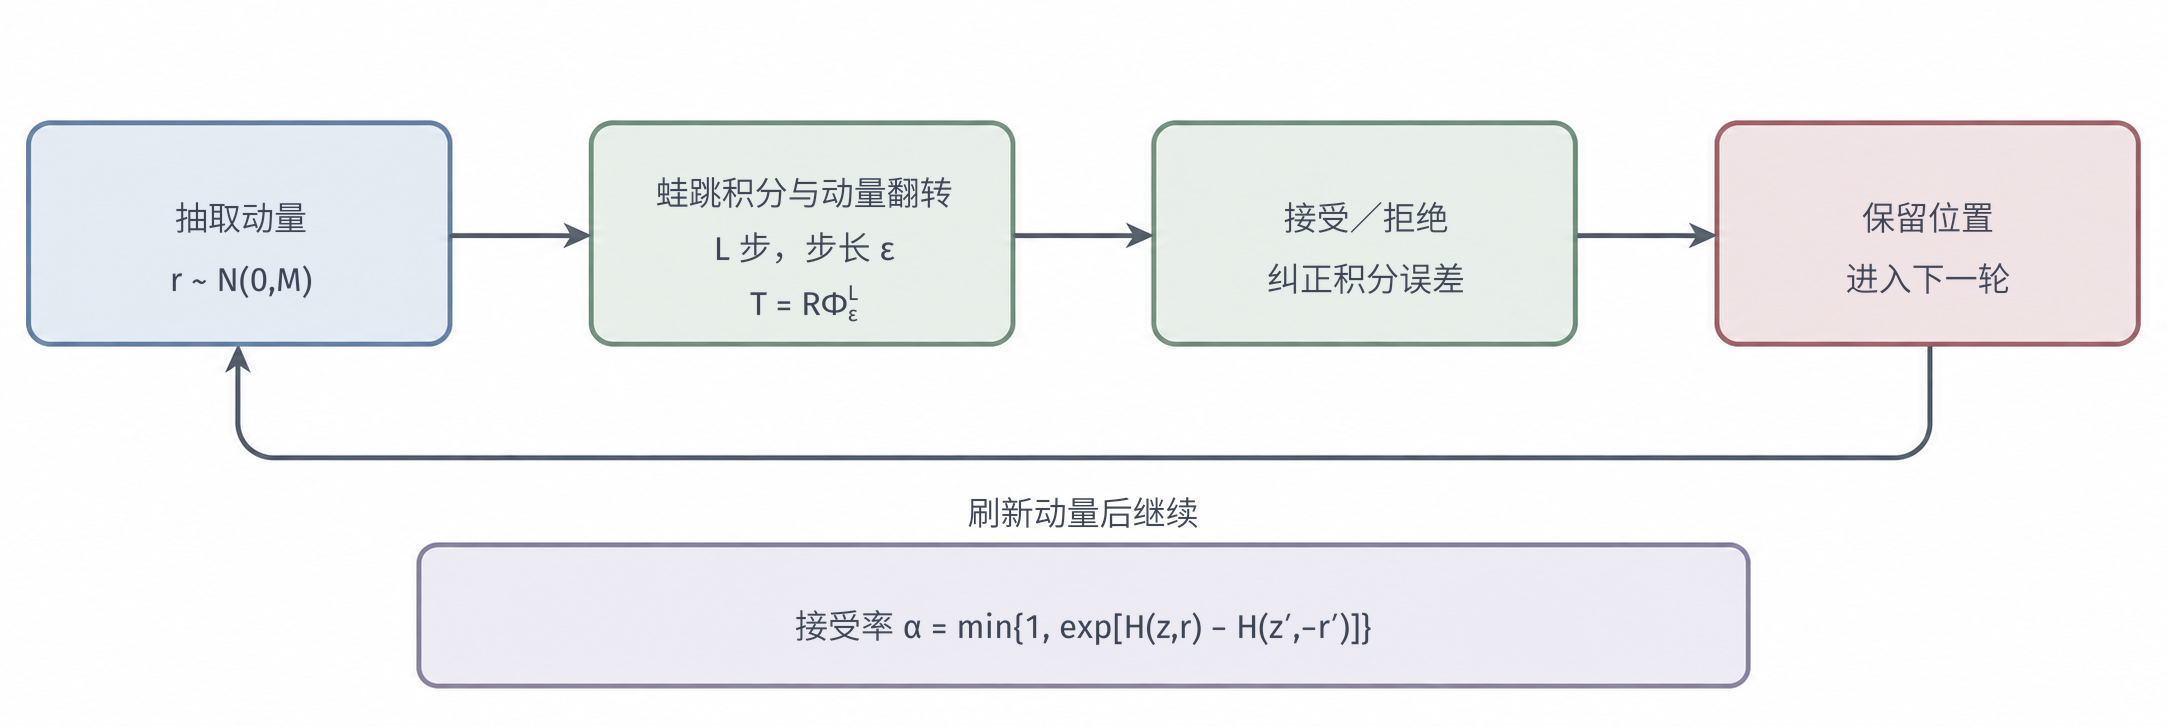
\includegraphics[width=169.000mm]{figures/06-probabilistic-graphical-models/02-inference/generated/pgm-sampling-hmc/figure.png}
  \par\medskip
  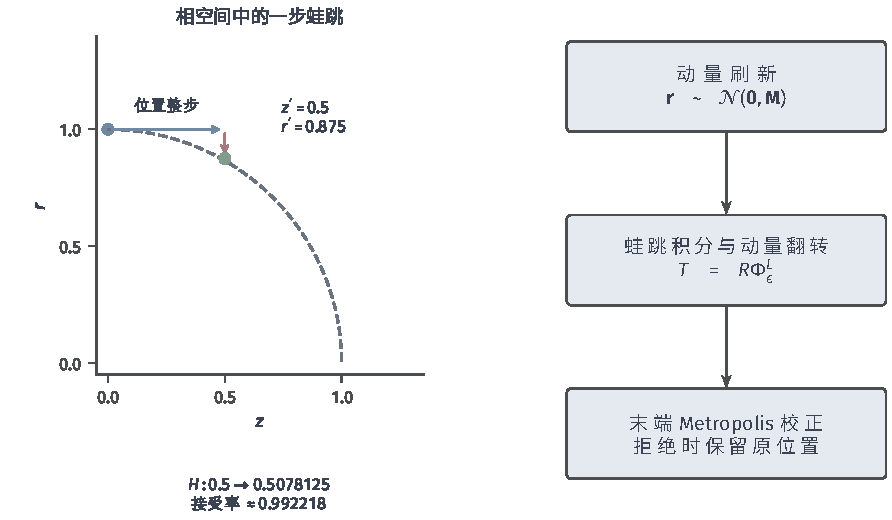
\includegraphics[width=142.118mm]{figures/06-probabilistic-graphical-models/02-inference/matplotlib/pgm-sampling-hmc/figure.pdf}
  \caption{HMC的更新流程与标准正态目标的一步数值计算。上方依次刷新动量、执行蛙跳并翻转末端动量、接受或拒绝提议、记录位置；$\bm z$是位置，$H$表示扩展状态的哈密顿量。下方的数值图由解析式生成：虚线圆弧属于$H=1/2$的精确轨迹，折线表示$\epsilon=0.5$的蛙跳整步与末端动量半步；初始动量半步因$z=0$不移动。动量翻转未画在相图上，接受率约为0.992218。}
  \label{fig:pgm-sampling-hmc}
\end{figure*}

步长$\epsilon$决定局部积分精度，轨迹长度$\tau=L\epsilon$决定一次提议运动多久。在足够光滑、数值稳定且$\tau$固定的条件下，蛙跳的全局状态误差为$O(\epsilon^2)$；在相应有界区域内，能量误差也可控制在这一阶。误差常数依赖曲率、维度和轨迹，采样误差还取决于链的探索。过大步长可能造成能量误差突然增大、非有限数值或拒绝；此类积分失败应拒绝并记录。过短轨迹探索不足，过长轨迹可能绕回原处，增加梯度计算却没有相应收益。

质量矩阵改变的是运动几何。为了看清它与目标尺度的关系，考虑高斯目标$\mathcal{N}(\bm{0},\bm{\Sigma})$，其中$\bm\Sigma$对称正定。此时$U(\bm z)=\tfrac12\bm z^{\top}\bm\Sigma^{-1}\bm z$加上常数，故$\nabla U(\bm z)=\bm\Sigma^{-1}\bm z$。由于$\bm M$固定，对位置方程再求一次导数，并代入动量方程，就得到
\[
  \frac{\mathrm{d}^2\bm{z}}{\mathrm{d}s^2}
     =\bm M^{-1}\frac{\mathrm d\bm r}{\mathrm ds}
     =-\bm{M}^{-1}\bm{\Sigma}^{-1}\bm{z}.
\]
按本章动量协方差等于$\bm M$的约定，取$\bm M=\bm\Sigma^{-1}$后，右侧变为$-\bm z$。每个坐标都满足$\mathrm d^2z_j/\mathrm ds^2=-z_j$，即频率为$1$的简谐运动；原来不同方向的快慢因而在人工时间下得到统一。软件中的“度量”和“逆质量”可能采用相反矩阵约定，使用时应先核对动量协方差与动能公式。固定矩阵补偿的是全局线性尺度；随位置变化的狭窄区域和多峰障碍需要其他几何或采样处理。通常在预热阶段调整尺度，正式保留样本时固定参数；任意依赖历史的持续调整不能直接套用上述齐次链证明。

若一次梯度求值成本为$C_{\nabla U}$，一轮HMC约需$O(L C_{\nabla U})$，另加动量生成和质量矩阵运算。对角矩阵的线性代数成本为$O(d)$每步，稠密矩阵通常为$O(d^2)$每步，并需预先分解。标准HMC不能直接更新离散变量；受约束连续变量常需先变换到无约束空间，并把变换的Jacobian加入密度。

计算出一条长轨迹也不保证位置移动有效。以标准正态和$M=1$的精确流为例，位置满足$z(s)=z(0)\cos s+r(0)\sin s$。若固定轨迹长度为$2\pi$，则不论本轮刷新出什么动量，末端位置都回到$z(0)$；精确积分的接受率虽为$1$，位置链却不移动。这就是固定长度与运动周期\term{共振}（resonance）妨碍遍历的一个最小例子。因此，积分误差控制之外仍需另外检查链的探索能力。

\section{序贯蒙特卡洛}
\label{sec:pgm-sampling-smc}

前面的MCMC针对“一个固定的后验分布”反复采样。但在很多实际问题里，观测是随时间一个接一个到来的（传感器持续上报、目标不断移动），目标分布每个时刻都在变；若每来一个观测就从头跑一条MCMC链，代价太高。自然的想法是让一群带权样本（粒子）随时间一起“向前走”，并在新观测到来时调整它们的权重。\term{序贯蒙特卡洛}（sequential Monte Carlo, SMC）复用上一阶段的样本及权重，逐步追踪一列目标分布。带权样本称为\term{粒子}（particle），每个粒子表示一个可能的潜在状态或状态历史。

为建立最小动态设定，令潜在状态为$\bm{z}_t$、观测为$\bm{x}_t$，真实时间$t=1,\ldots,T$写作下标。初始分布为$p(\bm{z}_1)$，转移分布为$p(\bm{z}_t\mid\bm{z}_{t-1})$，观测分布为$p(\bm{x}_t\mid\bm{z}_t)$。其联合分布分解为
\begin{equation}
  \begin{aligned}
    &p(\bm{z}_{1:T},\bm{x}_{1:T})\\
    &\qquad=p(\bm{z}_1)p(\bm{x}_1\mid\bm{z}_1)
       \prod_{t=2}^{T}
         p(\bm{z}_t\mid\bm{z}_{t-1})p(\bm{x}_t\mid\bm{z}_t).
  \end{aligned}
  \label{eq:pgm-sampling-state-space}
\end{equation}
这里假设给定上一潜状态后，更早状态不再影响当前状态；给定当前潜状态后，当前观测不再依赖其余变量。\term{滤波}（filtering）的目标是$p(\bm{z}_t\mid\bm{x}_{1:t})$，只利用截至当前的观测估计当前状态。若利用未来观测估计过去状态，则是平滑问题。本节只建立粒子计算所需的模型；第~\ref{sec:pgm-dynamic-common}节将从动态有向分解系统建立这些查询，第~\ref{sec:pgm-dynamic-continuous}节再比较何时可以用解析滤波代替粒子近似。

SMC不只适用于物理时间。一列$\gamma_\ell(\bm{z})=p(\bm{z})p(\bm{x}\mid\bm{z})^{\beta_\ell}$，其中$0=\beta_0<\cdots<\beta_L=1$，也可让粒子逐步从先验迁移到后验。这里的$\beta_\ell$是似然的指数，通常称为逆温度参数；指数从$0$增至$1$，表示逐步增强同一组观测对目标的影响，而不是增加新的观测。设各阶段归一化常数有限且为正，先验阶段按$\gamma_0=p(\bm z)$定义。对已有粒子，相邻阶段在其取值处的目标比为
\[
  \frac{\gamma_\ell(\bm z)}{\gamma_{\ell-1}(\bm z)}
    =p(\bm x\mid\bm z)^{\beta_\ell-\beta_{\ell-1}},
\]
其中比值只在前一阶段目标为正的位置计算；零似然位置在正指数阶段得到零权重。粒子据此更新权重，再按需要重采样，并进行保持当前归一化目标的MCMC移动。权重负责相邻目标的改变，MCMC核则在目标固定的当前阶段移动粒子。这里的$\ell$标记逆温度递增的算法阶段，与观测时间不同。本节以\term{粒子滤波}（particle filtering）为主，即用SMC近似式~\eqref{eq:pgm-sampling-state-space}的滤波分布。

\subsection{序贯重要性采样}
\label{sec:pgm-sampling-sis}

序贯重要性采样（SIS）就是把重要性采样改造成可随时间递推的形式：旧粒子继续保留，每步只需让它按状态转移“向前走一步”，再用新观测更新权重，而不必重算整条路径。路径后验涉及截至当前的全部潜状态，路径中的潜状态数量随时间增长。利用Markov分解，可以保留旧路径，只生成当前状态并更新权重。\term{序贯重要性采样}（sequential importance sampling, SIS）把路径提议写成
\[
  q_{1:t}(\bm{z}_{1:t}\mid\bm{x}_{1:t})
    =q_1(\bm{z}_1\mid\bm{x}_1)
      \prod_{s=2}^{t}
        q_s(\bm{z}_s\mid\bm{z}_{1:s-1},\bm{x}_{1:s}),
\]
其中每个$q_s$保持该阶段生成路径时所用的规则，使旧路径的提议密度仍由同一公共前缀表示。选择未归一化路径目标$\gamma_t=p(\bm{z}_{1:t},\bm{x}_{1:t})$。对$t\geq2$，新目标与新提议分别等于旧前缀乘上一个当前因子：
\[
  \begin{aligned}
    \gamma_t(\bm z_{1:t})
      &=\gamma_{t-1}(\bm z_{1:t-1})
          p(\bm z_t\mid\bm z_{t-1})p(\bm x_t\mid\bm z_t),\\
    q_{1:t}(\bm z_{1:t}\mid\bm x_{1:t})
      &=q_{1:t-1}(\bm z_{1:t-1}\mid\bm x_{1:t-1})
          q_t(\bm z_t\mid\bm z_{1:t-1},\bm x_{1:t}).
  \end{aligned}
\]
把两行相除，旧目标与旧提议的比值正是上一时刻的路径权重。因而不必重新计算整条路径的所有因子，只需保留旧权重，再乘新增目标因子与新增提议因子的比值。逐粒子写出这一关系，得到
\begin{equation}
  \begin{aligned}
    w_{1,i}&=
      \frac{p(\bm{z}_{1,i})p(\bm{x}_1\mid\bm{z}_{1,i})}
           {q_1(\bm{z}_{1,i}\mid\bm{x}_1)},\\
    w_{t,i}&=w_{t-1,i}
      \frac{p(\bm{z}_{t,i}\mid\bm{z}_{t-1,i})
            p(\bm{x}_t\mid\bm{z}_{t,i})}
           {q_t(\bm{z}_{t,i}\mid\bm{z}_{1:t-1,i},\bm{x}_{1:t})}.
  \end{aligned}
  \label{eq:pgm-sampling-sis-weight}
\end{equation}
下标$i=1,\ldots,n$标记粒子，$\bm{z}_{1:t,i}$是第$i$条路径。提议必须覆盖其对应的目标条件支撑集。权重的绝对尺度对归一化均值无影响，因此递推时可用上一时刻的归一化权重，再统一归一化当前权重。

路径后验中关于当前状态的查询，只使用$h(\bm z_t)$，与同一路径上更早坐标的具体记法无关。把路径经验分布对旧坐标边缘化，就相当于保留每条路径的权重和末端位置；这个操作不会把原来的不同权重自动变为等权。只保留路径末端，就得到滤波分布的经验近似
\begin{equation}
  \begin{aligned}
    \widehat p_t(\mathrm{d}\bm{z})
      &=\sum_{i=1}^{n}\bar w_{t,i}\delta_{\bm{z}_{t,i}}(\mathrm{d}\bm{z}),\\
    \widehat I_{t,h}&=\sum_{i=1}^{n}\bar w_{t,i}h(\bm{z}_{t,i}).
  \end{aligned}
  \label{eq:pgm-sampling-particle-measure}
\end{equation}
其中$\delta_{\bm{z}_{t,i}}$是把全部概率质量放在该粒子位置的点质量分布，不是连续密度曲线。若连续目标没有点质量，则有限粒子近似与它不可能在总变差距离下趋近。为看清这一点，取本次全部粒子位置组成的有限集合$B_n$：经验分布对$B_n$赋予概率$1$，无原子的目标却对$B_n$赋予概率$0$。按事件概率差的上确界定义，两者的总变差距离每次都是$1$。即使$n$增加，这个可随样本改变的有限集合仍能把两者区分开。因此，通常讨论的是适当测试函数$h$的积分是否收敛；这并不要求经验分布在总变差下收敛，也不把有限粒子解释为平滑的后验密度。

最简单的提议是模型转移$q_t=p(\bm{z}_t\mid\bm{z}_{t-1})$，此时新权重只是旧权重乘以当前观测似然。传播时尚未利用$\bm{x}_t$，所以新观测极具信息时，可能生成许多观测似然很低的候选。对预测似然有限且为正的父粒子，更有针对性的提议是
\begin{equation}
  \begin{aligned}
    q_t^\star(\bm{z}_t\mid\bm{z}_{t-1},\bm{x}_t)
      &=\frac{p(\bm{z}_t\mid\bm{z}_{t-1})
                p(\bm{x}_t\mid\bm{z}_t)}
              {p(\bm{x}_t\mid\bm{z}_{t-1})},\\
    p(\bm{x}_t\mid\bm{z}_{t-1})
      &=\int p(\bm{x}_t\mid\bm{z}_t)
             p(\bm{z}_t\mid\bm{z}_{t-1})\,\mathrm{d}\bm{z}_t.
  \end{aligned}
  \label{eq:pgm-sampling-optimal-proposal}
\end{equation}
它使式~\eqref{eq:pgm-sampling-sis-weight}中的增量变成只依赖父粒子的$p(\bm{x}_t\mid\bm{z}_{t-1,i})$，因而在给定父粒子的条件下，增量权重方差为零。这个“最优”只针对一步条件方差：不同父粒子的预测似然和旧权重仍可能不同，且$q_t^\star$本身可能难以计算或抽样。预测似然为零的父粒子对当前未归一化目标没有贡献，此时式中的条件提议无定义。

不重采样的SIS会把许多个增量相乘。若少数路径持续更符合观测，其权重会逐步占据总和的大部分，其他粒子虽仍占用计算，却几乎不影响答案。这称为\term{权重退化}（weight degeneracy）。在对数尺度上累加权重，并减去最大对数权重后再指数化，可以防止数值下溢，却不能消除这种真实的统计退化。

\subsection{粒子滤波与重采样}
\label{sec:pgm-sampling-particle-filter}

SIS有个随时间必然恶化的毛病：权重不断连乘，几步之后少数粒子会占据几乎全部权重，其余粒子形同虚设。一个自然的补救是“汰弱留强”——按权重概率性地复制好粒子、丢弃差粒子，使下一阶段的计算集中在更有希望的轨迹上。这就是重采样，加上它就成了粒子滤波。一个自然的补救是把下一轮计算资源更多地分给高权重粒子。\term{重采样}（resampling）按当前权重随机复制或淘汰粒子，把带权经验分布转成等权样本集合。若$N_i$为第$i$个原粒子的后代数，基本要求是
\begin{equation}
  \sum_i N_i=n,\qquad
  \mathbb{E}[N_i\mid\mathcal{F}_t]=n\bar w_{t,i},
  \label{eq:pgm-sampling-offspring}
\end{equation}
其中$\mathcal{F}_t$表示重采样前已有的全部粒子信息。由此，
\[
  \mathbb{E}\left[
     \left.\frac1n\sum_i N_i h(\bm{z}_{t,i})\right|\mathcal{F}_t
  \right]
    =\sum_i\bar w_{t,i}h(\bm{z}_{t,i}).
\]
重采样保持当前经验估计的条件期望。单次复制后的估计仍有随机波动，得到的后代也共享原粒子及路径信息。

三种常见方法都可以通过累积权重$C_j=\sum_{i=1}^{j}\bar w_{t,i}$实现。给定$u\in(0,1)$，取最小的$j$使$C_j\geq u$，便选中原粒子$j$。差异只在如何选择$n$个$u$，见表~\ref{tab:pgm-sampling-resampling}。

\begin{table}[htbp]
  \centering
  \begin{tabularx}{\linewidth}{@{}lXX@{}}
    \toprule
    方法 & 均匀数的构造 & 主要性质\\
    \midrule
    多项式 & $n$个独立的$u_i\sim\operatorname{Uniform}(0,1)$ & 后代数服从多项式分布，条件方差易分析\\
    分层 & 各区间$((i-1)/n,i/n)$独立抽一个$u_i$ & 每层均被使用，估计的条件方差不高于多项式法\\
    系统 & 抽一个$u\sim\operatorname{Uniform}(0,1/n)$，令$u_i=u+(i-1)/n$ & 只需一个随机偏移，结果受粒子排列影响\\
    \bottomrule
  \end{tabularx}
  \caption{固定粒子数的三种重采样。分层法的方差比较针对相同加权粒子集合和相同测试函数；系统法的方差还取决于排列与函数，需分别比较。}
  \label{tab:pgm-sampling-resampling}
\end{table}

\term{多项式重采样}（multinomial resampling）在给定$\mathcal{F}_t$后独立选取$n$个祖先，其均值估计的条件方差是
\begin{equation}
  \frac1n\left[
    \sum_i\bar w_{t,i}h(\bm{z}_{t,i})^2
      -\left(\sum_i\bar w_{t,i}h(\bm{z}_{t,i})\right)^2
  \right].
  \label{eq:pgm-sampling-resampling-variance}
\end{equation}
\term{分层重采样}（stratified resampling）用独立分层均匀数消除层间抽样次数的随机波动。其方差优势可以在同一组固定粒子和同一函数$h$上直接看出。令$a(u)$为累积权重规则选出的祖先索引，$g(u)=h(\bm z_{t,a(u)})$，并将$(0,1)$分成$n$个等长区间$J_j$。记均匀数落在第$j$层时，$g$的均值和方差分别为$\mu_j$和$s_j^2$，再令$\mu=n^{-1}\sum_j\mu_j$。给定重采样前的粒子后，多项式法的每个定位点先随机选层、再随机选层内位置，全方差公式给出
\[
  \begin{aligned}
    \operatorname{Var}(\widehat I_{\mathrm{mult}}\mid\mathcal F_t)
      &=\frac{1}{n^2}\sum_{j=1}^n s_j^2
          +\frac{1}{n^2}\sum_{j=1}^n(\mu_j-\mu)^2,\\
    \operatorname{Var}(\widehat I_{\mathrm{strat}}\mid\mathcal F_t)
      &=\frac{1}{n^2}\sum_{j=1}^n s_j^2.
  \end{aligned}
\]
这里两种$\widehat I$都表示复制后的等权函数均值。分层法在每层独立抽取一次，固定了各层的抽样次数，因而去掉了第二个非负的层间均值方差项。这会使条件方差不高于多项式法。\term{系统重采样}（systematic resampling）则共用一个随机偏移，容易实现。选中位置因共享偏移而相关，其方差比较需要考虑粒子排列和测试函数，不能直接继承分层法的上述独立求和。两者的比较和系统法反例见Douc等人的分析\scite{pgm-sampling-douc2005}

\term{自举粒子滤波}（bootstrap particle filter）将提议选为模型状态转移。下面依次传播粒子、按观测加权、输出本时刻估计，并在权重集中时重采样。也可以先重采样再传播，此时祖先提议及权重递推应与该顺序匹配。

\begin{algorithm}[带阈值重采样的自举粒子滤波]
  \label{alg:pgm-sampling-bootstrap}
  \begin{algorithmic}[1]
    \Require 状态空间模型、观测$\bm{x}_{1:T}$与时刻数$T\geq1$，查询函数$h$
    \Require 粒子数$n\geq1$，其中$n,T$为整数；阈值$\eta\in(0,1]$及重采样方案
    \Ensure 各时刻的滤波期望估计$\widehat I_{t,h}$
    \For{$t=1,\ldots,T$}
      \For{$i=1,\ldots,n$}
        \If{$t=1$}
          \State 抽取$\bm{z}_{1,i}\sim p(\bm{z}_1)$，置$v_i=1/n$
        \Else
          \State 抽取$\bm{z}_{t,i}\sim p(\bm{z}_t\mid\bm{z}_{t-1,i})$
          \State 置$v_i=\bar w_{t-1,i}$
        \EndIf
        \State $w_{t,i}\gets v_i p(\bm{x}_t\mid\bm{z}_{t,i})$
      \EndFor
      \State 若权重全零，报告本轮退化并停止；否则归一化为$\bar w_{t,i}$
      \State 输出$\widehat I_{t,h}=\sum_i\bar w_{t,i}h(\bm{z}_{t,i})$
      \If{$1/\sum_i\bar w_{t,i}^2<\eta n$且$t<T$}
        \State 按所选方案和$\bar w_{t,1:n}$抽取祖先索引$a_{t,1:n}$
        \State 同时复制旧$\bm{z}_{t,a_{t,i}}$为新$\bm{z}_{t,i}$，置$\bar w_{t,i}=1/n$
      \EndIf
    \EndFor
  \end{algorithmic}
\end{algorithm}

算法输入的$h$应是目标滤波分布下期望有定义的查询，$n$始终表示每轮粒子数，$T$表示输入观测的时刻数；它们不表示同一条MCMC链的运行长度。模型应能在生成粒子的位置给出非负有限的观测似然；若出现非有限值，应先报告模型或数值计算失败，不能把它作为有效权重继续归一化。所选重采样方案至少应满足式~\eqref{eq:pgm-sampling-offspring}的固定总后代数与条件后代均值。多项式、分层或系统方案均有前述构造，但其依赖结构和方差性质不同，不能只凭该均值条件就直接套用同一个中心极限定理。

阈值中的$1/\sum_i\bar w_{t,i}^2$衡量当前权重的集中程度，其含义和局限将在第~\ref{sec:pgm-sampling-diagnostics}节说明。重采样增加当前估计的随机性，多项式法的条件方差由式~\eqref{eq:pgm-sampling-resampling-variance}给出，所以算法先输出当前加权估计，再为后续传播重新分配粒子。权重全零时，归一化的粒子估计尚未定义，应检查提议覆盖、观测模型及粒子数，记录本轮退化。

\begin{example}[二状态设备的粒子滤波]
  \label{ex:pgm-sampling-filter}
  为单独观察时间递推，另设一个二状态教学模型。$Z_t\in\{0,1\}$表示当前故障状态，$X_t\in\{0,1\}$表示传感器读数。设
  \[
    \begin{aligned}
      p(Z_1=1)&=0.1,\\
      p(Z_t=1\mid Z_{t-1}=1)&=0.8,&
      p(Z_t=1\mid Z_{t-1}=0)&=0.1,\\
      p(X_t=1\mid Z_t=1)&=0.8,&
      p(X_t=1\mid Z_t=0)&=0.2.
    \end{aligned}
  \]
  收到$x_1=x_2=1$。精确滤波给出
  \[
    \begin{aligned}
      p(Z_1=1\mid x_1=1)&=\frac{0.1\times0.8}{0.1\times0.8+0.9\times0.2}
        =\frac4{13},\\
      p(Z_2=1\mid x_1=1)&=0.8\frac4{13}+0.1\frac9{13}
        =\frac{41}{130},\\
      p(Z_2=1\mid x_1=x_2=1)&=\frac{0.8\times41}{0.8\times41+0.2\times89}
        =\frac{164}{253}\approx0.648221.
    \end{aligned}
  \]
  假设上一轮已经得到等权粒子，传播到$t=2$的四个候选恰为$(0,1,1,0)$。其似然为$(0.2,0.8,0.8,0.2)$，归一化权重为$(0.1,0.4,0.4,0.1)$，故重采样前故障概率估计为$0.8$。

  用系统重采样，取偏移$u=0.05$，四个定位点为$0.05,0.30,0.55,0.80$；累积权重为$0.1,0.5,0.9,1$，因而祖先索引为$(1,2,3,3)$，新粒子为$(0,1,1,1)$。这次等权估计为$0.75$，不同于重采样前的$0.8$和精确答案。式~\eqref{eq:pgm-sampling-offspring}只保证对随机偏移再取期望后保持重采样前估计。
\end{example}

图~\ref{fig:pgm-sampling-resampling}展示第$3$个粒子被复制两次的过程。两个后代在复制瞬间相同，也共享过去的路径；后续随机转移可以分散当前位置，复制本身则无法恢复已经丢失的历史。\term{样本贫化}（sample impoverishment）指不同状态或祖先数量减少，它与权重集中对应不同的损失。状态噪声较小时，频繁重采样可能加重贫化；高维观测还可能使许多粒子的似然同时接近零。

\begin{figure}[htbp]
  \centering
  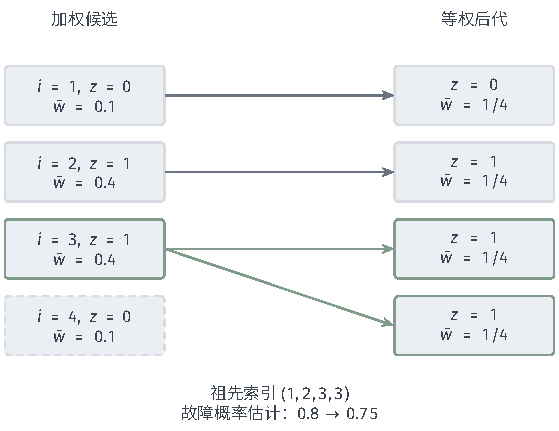
\includegraphics[width=94.650mm]{figures/06-probabilistic-graphical-models/02-inference/tikz/pgm-sampling-resampling/figure.pdf}
  \caption{二状态例子的系统重采样。左侧为四个带权候选，右侧为等权后代；连线标明复制来源。候选$4$没有后代，候选$3$被复制两次。后代等权，但状态及祖先多样性仍由复制来源决定。}
  \label{fig:pgm-sampling-resampling}
\end{figure}

若一次传播及似然计算成本分别为$C_{\mathrm{tr}},C_{\mathrm{obs}}$，一轮基础滤波成本约为$O(n(C_{\mathrm{tr}}+C_{\mathrm{obs}}))$，再加重采样成本。分层和系统法可沿累积权重单次扫描，在$O(n)$时间内完成；多项式法可用累积分布二分查找得到$O(n\log n)$实现，也有预处理后线性总成本的实现。只保存当前$d$维状态需$O(nd)$空间，保存所有粒子历史则随$T$增长。增加粒子数可改善固定时刻近似，长期平滑和高维滤波的效率还取决于路径与权重退化。

\subsection{Rao--Blackwell化粒子滤波}
\label{sec:pgm-sampling-rbpf}

粒子滤波对每个状态都要采样。若模型中一部分状态在给定其余状态时恰好有解析的条件分布（典型如离散模式下的连续状态服从线性高斯），就没必要也对它们采样——可以对这部分做精确Kalman递推，只对真正难处理的模式采样。这相当于在粒子滤波里再做一次Rao–Blackwell化。潜状态具有可解析的条件结构时，可以把随机计算集中到其余部分。\term{Rao--Blackwell化粒子滤波}（Rao--Blackwellized particle filtering, RBPF）只采样难以积分的状态部分，同时为每条粒子路径维护其余状态的条件分布。设$\bm{z}_t=(\bm{b}_t,\bm{u}_t)$，有
\begin{equation}
  \begin{aligned}
    &p(\bm{b}_{1:t},\bm{u}_t\mid\bm{x}_{1:t})\\
    &\qquad=p(\bm{b}_{1:t}\mid\bm{x}_{1:t})
        p(\bm{u}_t\mid\bm{b}_{1:t},\bm{x}_{1:t}).
  \end{aligned}
  \label{eq:pgm-sampling-rbpf-factor}
\end{equation}
若第二项可用有限维参数精确递推，则粒子只表示$\bm{b}_{1:t}$，每个粒子附带一份描述$\bm{u}_t$的解析状态。估计$h(\bm{b}_t,\bm{u}_t)$时，使用其条件期望
\[
  \widehat I_{t,h}^{\mathrm{RB}}
    =\sum_i\bar w_{t,i}
      \int h(\bm{b}_{t,i},\bm{u})
       p(\bm{u}\mid\bm{b}_{1:t,i},\bm{x}_{1:t})\,\mathrm{d}\bm{u}.
\]
查询中的条件分布已经使用当前观测$\bm x_t$，粒子加权却需要先计算看到该观测的概率。为区分这两个时刻，给定一条已扩展到$t$的模式路径，记
\[
  \begin{aligned}
    \pi_t^-(\bm u)
      &=p(\bm u_t=\bm u\mid\bm b_{1:t},\bm x_{1:t-1}),\\
    \ell_t(\bm b_{1:t})
      &=\int p(\bm x_t\mid\bm b_{1:t},\bm u)
                \pi_t^-(\bm u)\,\mathrm d\bm u.
  \end{aligned}
\]
这里$\pi_t^-$是当前观测进入之前的条件预测密度，$\ell_t$则是把连续状态积分掉后的预测观测密度。若$0<\ell_t<\infty$，看到$\bm x_t$后的条件密度才由Bayes公式给出：
\[
  \pi_t^+(\bm u)
    =\frac{p(\bm x_t\mid\bm b_{1:t},\bm u)\pi_t^-(\bm u)}
           {\ell_t(\bm b_{1:t})}.
\]
因此，查询积分使用$\pi_t^+$，权重计算使用$\pi_t^-$。把更新后的$\pi_t^+$再次当成预测分布来加权，会把同一次观测的影响重复算入。

模式路径本身也需要匹配提议。记模型在已有路径下的模式预测分布为
$a_t(\bm b_t)=p(\bm b_t\mid\bm b_{1:t-1},\bm x_{1:t-1})$，模式提议为$q_t^b(\bm b_t\mid\bm b_{1:t-1},\bm x_{1:t})$。对$t\geq2$，目标路径增加的因子为$a_t(\bm b_t)\ell_t(\bm b_{1:t})$，所以相应增量权重为
\[
  w_{t,i}\ \propto\ \bar w_{t-1,i}
    \frac{a_t(\bm b_{t,i})}
         {q_t^b(\bm b_{t,i}\mid\bm b_{1:t-1,i},\bm x_{1:t})}
    \ell_t(\bm b_{1:t,i}).
\]
比例常数在该轮粒子之间相同，重采样后的旧权重则按前述规则置为$1/n$。提议仍须覆盖有正目标贡献的模式；若模式按独立于连续状态的Markov链转移，则$a_t$简化为$p(\bm b_t\mid\bm b_{t-1})$。选择这一模式转移作为提议时，分式抵消，增量只剩积分预测似然；选择利用当前观测的其他模式提议时，分式必须保留。初始时刻同样使用模式先验与初始提议之比，并乘对应的初始积分观测密度。

典型例子是给定离散模式$b_t$后，连续状态服从线性高斯模型。每条模式路径维护高斯均值与协方差，通过Kalman递推完成条件滤波；模式仍用粒子表示。用标量的一步更新说明这一计算：给定某条模式路径及过去观测，连续状态预测分布为$U_t\sim\mathcal{N}(m^-,v^-)$，其中$v^->0$；观测满足$X_t=U_t+\varepsilon_t$，$\varepsilon_t\sim\mathcal{N}(0,\sigma_x^2)$，$\sigma_x^2>0$且噪声与$U_t$条件独立。预测观测是两个独立高斯量之和，故均值仍为$m^-$，方差为$v^-+\sigma_x^2$。这一步对未知$U_t$积分，也就是高斯卷积，得到用于模式权重的预测似然。

接着固定已经看到的$x_t$，更新连续状态。将先验预测密度与似然相乘，关于$u$的指数为
\[
  -\frac12\left[
       \left(\frac1{v^-}+\frac1{\sigma_x^2}\right)u^2
       -2\left(\frac{m^-}{v^-}+\frac{x_t}{\sigma_x^2}\right)u
       \right]+\text{与$u$无关的项}.
\]
因此，后验精度为$1/v_t=1/v^-+1/\sigma_x^2$，均值满足$m_t=v_t(m^-/v^-+x_t/\sigma_x^2)$。把分母通分，再把均值写成“预测均值加观测残差修正”的形式，便得到
\begin{equation}
  \begin{aligned}
    &p(x_t\mid b_{1:t},x_{1:t-1})
       =\mathcal{N}(x_t;m^-,v^-+\sigma_x^2),\\
    &k_t=\frac{v^-}{v^-+\sigma_x^2},\\
    &m_t=m^-+k_t(x_t-m^-),\qquad v_t=(1-k_t)v^-.
  \end{aligned}
  \label{eq:pgm-sampling-rbpf-gaussian}
\end{equation}
第一行对应观测前的积分预测似然，用于粒子权重；后两行给出观测后的条件高斯参数，用于查询和下一轮预测。$k_t$是标量Kalman增益，控制当前观测对条件均值的修正幅度：预测方差相对于观测噪声越大，当前残差得到的权重越大。上述卷积与配方承担不同计算，不能把观测后的条件高斯再次代入同一次预测似然。

假设两个等先验模式分别给出$U_t\sim\mathcal{N}(0,1)$和$\mathcal{N}(0,4)$，共同观测噪声方差$\sigma_x^2=1$，观测$x_t=1$。两模式的预测似然分别为$\mathcal{N}(1;0,2)\approx0.219696$和$\mathcal{N}(1;0,5)\approx0.161434$，归一化模式权重约为$0.576433,0.423567$。更新后的连续状态分别服从$\mathcal{N}(0.5,0.5)$和$\mathcal{N}(0.8,0.8)$，故混合均值约为$0.627070$。连续状态通过两个条件高斯表示，均值可直接积分，同时保留条件不确定性。从这些高斯额外抽样再估计均值，会引入额外的条件抽样波动。

RBPF利用可精确递推的条件分布减少随机性，但每个粒子需要存储协方差并进行矩阵运算，模式路径也可能退化。若用扩展Kalman等近似替代精确条件积分，结果中还包含条件滤波的近似误差。全方差公式解释相容条件化下的方差缩减；相同运行时间下的整体收益，则需比较粒子数、重采样和解析运算成本。Doucet等人的工作详细讨论了这一构造\scite{pgm-sampling-doucet2000}。

\section{算法分析}
\label{sec:pgm-sampling-analysis}

采样估计是否可信，需要同时说明目标、渐近规模与有限计算误差。渐近正确不代表有限时间内准确，不同机制的误差来源也不同：独立样本看权重和矩，MCMC看链的相关性与遍历性，粒子滤波还要看权重退化和祖先多样性。保持正确目标的核可能因探索缓慢而给出不可靠的有限估计，有有限样本偏差的比值估计也可能随样本数趋于一致。下面先逐一建立独立样本、加权样本、链与粒子的极限条件，再讨论能够从有限输出中直接检查的诊断量。

\subsection{一致性、偏差与方差}
\label{sec:pgm-sampling-consistency}

独立直接采样的条件最清楚。对固定查询$h$，独立同分布与$\mathbb{E}_p|h|<\infty$给出强一致性；$\mathbb{E}_p h^2<\infty$进一步给出式~\eqref{eq:pgm-sampling-iid-clt}的方差与中心极限定理。对于有界指示函数，这些矩条件自动成立。对于Cauchy等重尾分布，某些均值不存在，此时需要选择有定义的查询量。$n^{-1/2}$误差尺度也只描述随机计算误差，不包括模型失配。

重要性采样把这些矩条件移到了$q$下的加权函数。归一化目标的普通IS需要$r h$可积；有限方差与普通中心极限定理需要$\mathbb{E}_q(rh)^2<\infty$。SNIS的一致性条件见式~\eqref{eq:pgm-sampling-snis}之后。为了得到一个方便使用的SNIS中心极限定理，仍令候选独立来自固定$q$，要求目标支撑被覆盖、$0<Z_{\bm x}=\mathbb E_qw<\infty$，并进一步要求$\mathbb{E}_q w^2<\infty$和$\mathbb{E}_q(wh)^2<\infty$。

先把比值中同时变化的两部分写清。令$Y_i=w_i h(\bm z_i)$、$\bar Y_n=n^{-1}\sum_iY_i$与$\bar W_n=n^{-1}\sum_iw_i$，则$\widehat I_{h,n}^{\mathrm{SNIS}}=\bar Y_n/\bar W_n$，而$\mu_Y=\mathbb E_qY=Z_{\bm x}I_h$。记$\Delta_Y=\bar Y_n-\mu_Y$和$\Delta_W=\bar W_n-Z_{\bm x}$。联合中心极限定理使这两个偏差均为$O_{\mathbb P}(n^{-1/2})$；$\bar W_n$则依概率趋向严格正的$Z_{\bm x}$，所以分母为正的概率趋于$1$。有限样本的全零权重仍应按前文报告，不能输出归一化估计；讨论渐近分布时，可在这类事件上任意补定一个固定值，因为该事件概率趋零，不改变下面的分布极限。函数$f(a,b)=a/b$在该点对分子、分母的导数分别为$1/Z_{\bm x}$和$-I_h/Z_{\bm x}$，因而一阶展开为
\[
  \begin{aligned}
    \widehat I_{h,n}^{\mathrm{SNIS}}-I_h
      &=\frac{\Delta_Y-I_h\Delta_W}{Z_{\bm x}}
           +o_{\mathbb P}(n^{-1/2}),\\
    \Delta_Y-I_h\Delta_W
      &=\frac1n\sum_{i=1}^n w_i\bigl(h(\bm z_i)-I_h\bigr).
  \end{aligned}
\]
第二行利用$\mu_Y=Z_{\bm x}I_h$抵消常数项。它表明分母波动与分子波动共同形成中心化贡献，并且$\mathbb E_q[w(h-I_h)]=0$。对这个贡献应用独立样本中心极限定理，得到
\begin{equation}
  \begin{aligned}
    \sqrt n(\widehat I_{h,n}^{\mathrm{SNIS}}-I_h)
       &\xrightarrow{\mathrm{d}}\mathcal{N}(0,v_h^{\mathrm{IS}}),\\
    v_h^{\mathrm{IS}}
       &=\frac{\mathbb{E}_q[w^2(h-I_h)^2]}{Z_{\bm{x}}^2}.
  \end{aligned}
  \label{eq:pgm-sampling-snis-clt}
\end{equation}
关键的一阶随机量是$w(h-I_h)$，不是单独的$w$。这解释了为什么同一组权重对于不同查询可能具有不同精度。

SNIS的偏差也可由同一个比值展开看清，但这次需要控制取期望后的余项，只有一阶的依概率结论还不够。为简化书写，在以下展开中暂记$Z=Z_{\bm x}$。将$f(a,b)=a/b$在$(\mu_Y,Z)$处展开到二阶，得到
\[
  \begin{aligned}
    \widehat I_{h,n}^{\mathrm{SNIS}}-I_h
      &=\frac{\Delta_Y-I_h\Delta_W}{Z}\\
      &\quad-\frac{\Delta_Y\Delta_W}{Z^2}
         +\frac{I_h\Delta_W^2}{Z^2}+R_n,\\
    R_n&=\frac{\Delta_W^2(\Delta_Y-I_h\Delta_W)}
                  {Z^2\bar W_n}.
  \end{aligned}
\]
这里写出的$R_n$在$\bar W_n>0$时还是精确的余项表达。若在全零权重事件上将估计量补定为常数$c_0$，也应在该事件上把$R_n$定义为$c_0-I_h$。这是因为此时$\bar Y_n=\bar W_n=0$，已经显示的一阶和二阶项相互抵消，余项必须承接补定估计量与$I_h$的差。独立候选下，全零事件概率为$\mathbb P_q(w=0)^n$；由$\mathbb E_qw>0$可知$\mathbb P_q(w=0)<1$，所以这一补定对余项期望的贡献随$n$指数衰减，不改变下面的偏差阶。由于比值对分子线性，没有$\Delta_Y^2$项；分子与分母的交叉项带负号，反映分子固定时，分母增大会使比值减小。两个一次项的期望均为零，而独立候选给出
\[
  \mathbb E[\Delta_Y\Delta_W]
      =\frac{\operatorname{Cov}_q(wh,w)}n,\qquad
  \mathbb E[\Delta_W^2]=\frac{\operatorname{Var}_q(w)}n.
\]
在足够高阶矩和分母尾部控制使$\mathbb E R_n=o(n^{-1})$的条件下，对二阶展开取期望，便得到
\begin{equation}
  \mathbb{E}[\widehat I_{h,n}^{\mathrm{SNIS}}]-I_h
    =\frac{I_h\operatorname{Var}_q(w)-\operatorname{Cov}_q(wh,w)}
            {n Z_{\bm{x}}^2}+o(n^{-1}).
  \label{eq:pgm-sampling-snis-bias}
\end{equation}
例如$w\geq a>0$且$\mathbb{E}_q[w^4+|wh|^4]<\infty$，是控制分母和展开余项的一组较强充分条件。此时$\bar W_n\geq a$，两个样本均值偏差的二阶矩为$O(n^{-1})$、四阶矩为$O(n^{-2})$。将这些界代入$R_n$并使用Cauchy--Schwarz不等式，可得$\mathbb E|R_n|=O(n^{-3/2})=o(n^{-1})$。因此，常见的$O(n^{-1})$偏差来自交叉协方差与分母方差，而不是无条件的比值性质；这一阶数所需的余项和分母控制，比一致性所需的可积性与支持覆盖更强。

MCMC考察运行长度增长时的时间平均，其中样本通常相关。先说明强大数定律涵盖哪些起点。设固定的齐次转移核$K$在所声明的状态空间或闭合Harris类上正Harris常返，并保持概率分布$p$。对实值且满足$\mathbb E_p|h|<\infty$的$h$，从该类中的任意初始状态出发，时间平均都几乎必然收敛到$I_h$。这里“任意”限定在已经声明具有该性质的类内；仅知道某个核保持$p$，不足以把另一个封闭类中的起点也包括进来。非周期性另用于保证每一步的分布收敛；上述时间平均结论本身不要求非周期性。

若链从平稳分布启动，有限样本均值在期望存在时仍无偏，只是有相关性；从指定点启动时，有限预热用于减轻初值影响，剩余的初始化偏差还取决于核的混合速度。有限预热并不会把当前分布自动变成$p$，也不能替代一个结论所要求的起点条件。

MCMC中心极限定理还需额外条件。一组常用充分条件是\term{几何遍历性}（geometric ergodicity），即到平稳分布的距离按几何速率衰减，且允许系数依赖起点。具体地，在标准Borel状态空间上，设固定的齐次核$K$不可约、非周期且保持$p$，存在$0<a<1$及对$p$几乎处处起点有限的$C(\bm z)$，使
\[
  \lVert K^k(\bm z,\cdot)-p\rVert_{\mathrm{TV}}
    =\sup_B|K^k(\bm z,B)-p(B)|\leq C(\bm z)a^k.
\]
总变差距离在这里比较运行$k$步后的事件概率与目标事件概率，几何界控制两者相差的速率。标准Borel包括本章的欧氏空间及离散状态空间；这一可测性设定使常用条件分布和耦合论证能够适用。再要求某个$\delta>0$满足$\mathbb{E}_p|h|^{2+\delta}<\infty$，先从$\bm z^{(0)}\sim p$的平稳启动得到
\[
  \sqrt n(\widehat I_{h,n}-I_h)
     \xrightarrow{\mathrm{d}}\mathcal{N}(0,v_h^{\mathrm{MC}}).
\]
在上述一般几何遍历条件下，这个结论还可以扩展到$p$几乎处处的固定起点。这里允许排除$p$概率为零的异常起点。若进一步采用前面整类正Harris常返的设定，并保持非周期性，则该类中的每个起点都在总变差下收敛到$p$；将其与平稳链耦合，同一中心极限定理便可扩展到类内全部起点。这个扩展依据的是核在整类上的遍历性质，不是已经完成了有限预热。未被声明为该类成员的其他指定点，不能自动继承这个保证。

长期依赖的控制是推导正态误差分布所需的环节。再生方法把路径在特定随机返回时刻切成可以独立处理的完整区段，再控制初末不完整区段；Poisson方程方法则把中心化求和转为鞅差求和及可忽略的边界项，其中每个鞅差增量在给定过去信息时的条件均值为零。两者都需要证明相应矩和余项条件，不能只靠目标不变性得到正态误差。其他条件组合也可能建立中心极限定理，本章保留上述一组充分条件；更一般的证明以及从平稳启动扩展到$p$几乎处处固定起点的论证，见Roberts与Rosenthal的综述\scite{pgm-sampling-roberts2004}

SMC的样本数极限又不同：通常先固定一个有限时刻$t$，再令粒子数$n\to\infty$。为看清这一区别，可以考察一组较强而易检查的充分条件：初始粒子独立来自模型初始分布，传播使用正确的Markov转移；每个固定时刻的观测似然作为状态函数有正下界和有限上界；测试函数$h$有界；采用固定日程的多项式重采样。此时滤波积分估计一致，并满足适当的$\sqrt n$中心极限定理。一般提议需要相应的重要性权重矩条件，其他重采样方案和自适应日程还需要各自的方差与依赖条件，后代数条件无偏只是其中一项要求。

固定时刻一致性的证明思路是归纳。给定旧粒子后，新传播条件独立，因此对有界函数，传播抽样相对于其条件均值的方差为$O(1/n)$。条件均值是旧经验分布对转移后函数的积分，由归纳假设收敛。乘有界似然并除以远离零的归一化常数，仍保持收敛；多项式重采样再增加一个由式~\eqref{eq:pgm-sampling-resampling-variance}控制的$O(1/n)$条件方差。固定步数下反复使用这三个步骤便得到一致性。这是证明纲要，中心极限定理还需追踪每一代随机扰动如何传播，渐近方差包含历史各代贡献，而不只是当前粒子的样本方差\scite{pgm-sampling-chopin2004}

上述证明中的误差常数可以随$t$迅速增大。固定$n$让时间无限延长，与固定$t$让$n$趋向无穷，是不同的极限；要获得时间一致误差界，通常还需状态转移的遗忘或混合性质，以及适当的似然控制。归一化粒子滤波均值一般有有限$n$偏差。边缘似然却可以有无偏的粒子估计，因为它保留的是未归一化积分，而不是随机分母下的比值。

先把需要保存的尺度接回算法~\ref{alg:pgm-sampling-bootstrap}。记$g_t(\bm z)=p(\bm x_t\mid\bm z)$，传播后、归一化前的权重为$w_{t,i}=v_i g_t(\bm z_{t,i})$，其中$v_i$就是算法中的旧归一化权重，初始时为$1/n$。每轮归一化除掉的总和为
\begin{equation}
  \begin{aligned}
    \widehat c_t&=\sum_{i=1}^n v_i g_t(\bm z_{t,i}),\\
    \widehat Z_t&=\prod_{s=1}^t\widehat c_s,\qquad \widehat Z_0=1.
  \end{aligned}
  \label{eq:pgm-sampling-evidence-product}
\end{equation}
$\widehat c_t$近似预测观测密度$p(\bm x_t\mid\bm x_{1:t-1})$，$\widehat Z_t$近似边缘似然$p(\bm x_{1:t})$。初始时刻及上一轮已经重采样时$v_i=1/n$，因子是当前似然的粒子平均；上一轮未重采样时必须继续使用保留的非等权$v_i$。只保存归一化权重会丢掉这些总和。若为数值稳定对全部权重乘了共同尺度，计算$\widehat c_t$时还须还原该尺度，或在对数域保存对应的加数。

乘积的无偏性不能由“各因子分别无偏”推出，因为各轮使用的粒子相互依赖。可以直接对未归一化经验积分作条件递推。固定有限时刻和粒子数，先考虑初始独立模型采样、正确模型转移及每轮多项式重采样。观测似然非负有界、查询$h$有界，是使以下期望与积分均存在的一组充分条件。先约定：仅在截至当前每轮总权重都为正的存活事件上定义归一化经验积分；若某轮总权重为零，则直接把该运行的$\widehat Z_t$和$\Gamma_t^n(h)$定义为零，并在后续各轮维持为零，避免用零乘一个未定义的归一化积分。在存活分支上，令$\eta_t^n(h)$表示完成本轮可选重采样后的经验积分，$\Gamma_t^n(h)=\widehat Z_t\eta_t^n(h)$；未重采样时仍使用原来的加权积分。给定传播后的粒子，条件无偏的重采样使$\eta_t^n(h)$的条件均值等于$\sum_i\bar w_{t,i}h(\bm z_{t,i})$。因此，复制前的未归一化积分为
\[
  \widehat Z_{t-1}\sum_i v_i g_t(\bm z_{t,i})h(\bm z_{t,i}),
\]
复制后的$\Gamma_t^n(h)$在当前粒子信息下的条件期望与它相同；其中$\widehat c_t$恰好消去了归一化权重中的随机分母。对$t\geq2$，再对本轮传播取条件期望，有
\begin{equation}
  \begin{aligned}
    \mathbb E[\Gamma_t^n(h)\mid\mathcal F_{t-1}]
      &=\widehat Z_{t-1}\sum_i\bar w_{t-1,i}
          Q_t h(\bm z_{t-1,i}),\\
    Q_t h(\bm z)
      &=\int p(\bm z'\mid\bm z)g_t(\bm z')
                    h(\bm z')\,\mathrm d\bm z'.
  \end{aligned}
  \label{eq:pgm-sampling-evidence-recursion}
\end{equation}
这里$\mathcal F_{t-1}$包含上一轮重采样后的全部信息，$Q_t h$把一次状态转移、观测加权和当前查询合成一个旧状态的函数。含粒子状态与归一化权重的和式在对应存活分支上使用；若上一轮已经灭绝，递推两端都按零定义，无需再生成后续粒子。右侧正是$\Gamma_{t-1}^n(Q_t h)$。初始独立采样给出$\mathbb E\Gamma_1^n(h)=\int p(\bm z_1)g_1(\bm z_1)h(\bm z_1)\,\mathrm d\bm z_1$。据此逐轮取期望，便得到
\[
  \begin{aligned}
    \mathbb E\Gamma_t^n(h)
      &=\int h(\bm z_t)p(\bm z_t,\bm x_{1:t})\,\mathrm d\bm z_t,\\
    \mathbb E\widehat Z_t&=p(\bm x_{1:t}).
  \end{aligned}
\]
第二行取$h\equiv1$。它证明的是未归一化估计的无偏性；$\Gamma_t^n(h)/\widehat Z_t$仍有随机分母，因而不能据此判定滤波均值有限样本无偏。

若某轮权重全零，则当前滤波分布无法归一化，算法按原规则报告退化并停止。为了把证据估计定义在所有随机运行上，可将这种运行的$\widehat Z_t$及后续$\widehat Z_s$记为零，未归一化经验积分也记为零；此时不再要求定义对应的归一化滤波估计。零贡献必须保留在重复运行的平均中，不能丢弃失败运行、只对成功运行求平均后仍声称无偏。此前的一致性示例使用严格正下界，已经排除了全零事件；此处非负有界的设定则容许它出现。

按当前已有粒子信息决定是否重采样，例如算法中的权重ESS阈值，只要决策不使用未来随机量，且所选方案在该信息条件下仍保持后代均值，重采样或不重采样都保持同一个经验积分的条件期望，上述无偏递推仍可逐步应用。这个论证固定粒子数和要估计的时刻；任意改变粒子数、停止时刻、提议或目标的自适应规则需要重新核对权重与条件期望。即使某种自适应重采样保留了证据无偏性，其中心极限定理和方差公式也仍须满足该规则的额外条件。

\subsection{有效样本量与收敛诊断}
\label{sec:pgm-sampling-diagnostics}

估计精度既取决于样本数量，也取决于样本如何贡献以及如何相关。\term{有效样本量}（effective sample size, ESS）借独立样本的尺度描述这些影响。权重ESS衡量贡献集中，自相关ESS匹配具体查询的长期方差，两者需要分别解释。

先只考察归一化非负权重如何分配本批贡献。若恰有$m$个粒子各占$1/m$、其余为零，则平方权重和为$m(1/m)^2=1/m$，取倒数正好返回贡献相等的粒子数$m$。更一般地，按权重独立抽取两次索引，两次选中同一原粒子的概率为$\sum_i\bar w_i^2$。这一概率越大，权重越集中；其倒数用“等贡献粒子数”的尺度表示集中程度。由此引出常用的\term{权重有效样本量}（weight-based ESS）
\begin{equation}
  n_{\mathrm{eff}}^{w}
    =\frac{1}{\sum_i\bar w_i^2}
    =\frac{(\sum_i w_i)^2}{\sum_i w_i^2},
  \qquad 1\leq n_{\mathrm{eff}}^{w}\leq n.
  \label{eq:pgm-sampling-weight-ess}
\end{equation}
上下界来自非负性和Cauchy--Schwarz不等式：等权时等于$n$，一个权重占满总和时等于$1$。若候选确实独立来自固定$q$且$\mathbb{E}_q w^2<\infty$，大数定律还给出
\[
  \frac{n_{\mathrm{eff}}^{w}}{n}
    \longrightarrow
    \frac{(\mathbb{E}_q w)^2}{\mathbb{E}_q w^2}
    =\frac{1}{1+\operatorname{CV}_q(w)^2},
\]
其中$\operatorname{CV}_q(w)$为权重的标准差与均值之比。因此，权重ESS描述已抽到的贡献集中程度；对具体$h$的方差等价样本数，还需考虑函数值与权重的关系。真正的IS渐近方差还含有式~\eqref{eq:pgm-sampling-snis-clt}中的$(h-I_h)^2$。

表~\ref{tab:pgm-sampling-weight-example}中，$n_{\mathrm{eff}}^w=2.51^2/(0.01^2+0.9^2+0.9^2+0.7^2)\approx2.986$。这一数值只反映已抽到的权重，未访问的罕见状态仍需其他检查。粒子滤波例子重采样前的权重ESS为$1/(0.1^2+0.4^2+0.4^2+0.1^2)\approx2.941$，重采样后立即变成$4$；但图~\ref{fig:pgm-sampling-resampling}已经显示祖先反而减少。在SMC中，权重ESS主要帮助选择重采样时刻，滤波误差还需要考虑状态和祖先多样性。

MCMC常常所有样本等权，权重ESS因而为$n$。重复停留和缓慢移动带来的时间相关，需要通过样本均值的协方差分析。设链已平稳，$0<\sigma_h^2=\operatorname{Var}_p(h)<\infty$，令$\rho_h(\ell)$为$h(\bm{z}^{(k)})$与$h(\bm{z}^{(k+\ell)})$的相关系数。展开样本均值的协方差和，有
\begin{equation}
  \operatorname{Var}(\widehat I_{h,n})
    =\frac{\sigma_h^2}{n}
      \left[1+2\sum_{\ell=1}^{n-1}
          \left(1-\frac{\ell}{n}\right)\rho_h(\ell)\right].
  \label{eq:pgm-sampling-autocorrelation-variance}
\end{equation}
滞后$\ell$的样本对恰有$n-\ell$个，因而出现括号中的系数。若自相关绝对可和，定义\term{积分自相关时间}（integrated autocorrelation time）
\begin{equation}
  \tau_h=1+2\sum_{\ell=1}^{\infty}\rho_h(\ell),\qquad
  v_h^{\mathrm{MC}}=\sigma_h^2\tau_h,\qquad
  n_{\mathrm{eff},h}^{\mathrm{MC}}=\frac{n}{\tau_h}.
  \label{eq:pgm-sampling-mcmc-ess}
\end{equation}
这里假定$0<\tau_h<\infty$；还需前述中心极限定理条件，才能据此使用正态近似误差区间。$\tau_h$依赖函数$h$，故均值、尾概率和不同坐标通常有不同ESS；负相关还可能使$\tau_h<1$，此时ESS大于$n$，并不矛盾，因为它匹配的是估计方差而非独立点的实际数量。

例如平稳自回归序列的$\rho_h(\ell)=0.9^\ell$，则$\tau_h=1+2(0.9/0.1)=19$，$10000$次迭代对该查询只有约$526$个独立样本的渐近精度。对前述强相关高斯的Gibbs坐标，$\rho=0.99$给出的每轮相关系数为$0.9801$，对应$\tau_h=(1+0.9801)/(1-0.9801)\approx99.50$。两个例子将运行长度与该查询的渐近精度联系起来，高接受率仍可能伴随低有效样本量。简单地每隔若干步保留一个点虽然降低保留序列的相关性，也丢弃了已付费的计算；除非有存储或后续处理约束，稀疏保留不是改善采样效率的通用办法。

样本相关系数的高滞后估计噪声较大，不能把所有可计算滞后的样本相关系数直接相加。截断方法只累计到预先选定或按稳定规则选出的滞后，再检查截断位置改变时结论是否稳定；谱方差方法对样本自协方差施加随滞后衰减的窗权重，估计零频率处的长期波动尺度。批均值方法则把序列分成若干连续长批，使每批内部的相关都进入批均值，再用批间波动估计长期方差。

例如将$n$个保留的$h$值分为$a$个长为$b$的等长批，暂设$n=ab$，$a\geq2$。记第$j$批均值为$\bar H_j$、总均值为$\bar H$，可构造
\[
  \widehat v_h^{\mathrm{MC}}
    =\frac{b}{a-1}\sum_{j=1}^a(\bar H_j-\bar H)^2.
\]
若单批已经足够长，批均值的方差约为$v_h^{\mathrm{MC}}/b$，所以样本批方差乘以$b$对应所需的长期方差尺度。渐近使用时应让批长和批数都增长，并满足相应遍历与矩条件；前述中心极限定理本身不自动保证任意截断、窗宽或批长规则都一致。用$\sqrt{\widehat v_h^{\mathrm{MC}}/n}$报告具体查询的MCSE，可以把估计出的长期方差直接换回该查询的均值误差，而不是只报告一个全局ESS。

独立SNIS可以对式~\eqref{eq:pgm-sampling-snis-clt}作样本代入。在该式的覆盖与二阶矩条件下，以$\bar W_n$代替$Z_{\bm x}$、以$\widehat I_h$代替$I_h$，把期望代为样本平均，得到
\[
  \begin{aligned}
    \frac{\widehat v_h^{\mathrm{IS}}}{n}
       &=\frac{n^{-1}\sum_iw_i^2(h_i-\widehat I_h)^2}
               {n\bar W_n^2}\\
       &=\sum_i\bar w_i^2(h_i-\widehat I_h)^2,\\
    \widehat{\operatorname{MCSE}}(\widehat I_h)
       &=\left[\sum_i\bar w_i^2(h_i-\widehat I_h)^2\right]^{1/2},
       \qquad h_i=h(\bm z_i).
  \end{aligned}
\]
这里依赖候选独立与相应加权矩；若权重重尾到没有所需方差，代入一个有限数值不能恢复中心极限定理。共享祖先的粒子系统还包含额外依赖，不能直接把独立SNIS的式子当作其全部误差。SMC可通过多次独立运行整个粒子滤波比较估计波动，或采用专门的粒子方差估计。

单条链可能在一个局部区域内看起来很稳定。多链诊断从分散的有效初值运行若干条独立链，比较链内与链间变化。\term{$\widehat R$诊断}（R-hat diagnostic）用两种变化尺度之比发现不同链尚未探索相同分布的迹象。设共有$m\geq2$条链，每条保留$n\geq2$个函数值$h_{j,k}$，链均值为$\bar h_j=n^{-1}\sum_kh_{j,k}$，总体均值为$\bar h=m^{-1}\sum_j\bar h_j$，链内样本方差采用
\[
  s_j^2=\frac1{n-1}\sum_{k=1}^n(h_{j,k}-\bar h_j)^2.
\]
这里$n$表示每条链的保留长度，不是多条链合计长度。经典形式先计算链内平均方差$W$和按$n$放大后的链均值样本方差$B$，再构造
\begin{equation}
  \begin{aligned}
    W&=\frac1m\sum_{j=1}^{m}s_j^2,&
    B&=\frac{n}{m-1}\sum_{j=1}^{m}(\bar h_j-\bar h)^2,\\
    \widehat V&=\frac{n-1}{n}W+\frac{B}{n},&
    \widehat R&=\sqrt{\widehat V/W}.
  \end{aligned}
  \label{eq:pgm-sampling-rhat}
\end{equation}
$B/n$是各链均值之间的样本方差，$B$与$W$则都以单个函数值的方差为尺度。若各链已经近似探索同一分布且相关较弱，链均值方差约为单点方差除以$n$，所以$B$与$W$应大致相当；若链还停留在不同区域，链均值差异就可能使$B$明显增大。$\widehat V$将链内估计乘$(n-1)/n$，再补入链均值差异$B/n$，因而能够暴露只看链内波动遗漏的位置差异。样本相关与有限长度会影响这些估计，不能要求每次运行都恰有$\widehat R=1$。

该比值的通常解释要求$W>0$。所有链完全不动而使$W=0$时，比值无定义或缺少通常的尺度比较含义，应先检查链的移动，而不能将常数输出当成已经充分探索。

秩归一化的分裂诊断先把每条链的保留序列分成前后两半，并把各半段当成单独链。两半的位置差异因而能进入链间比较，帮助发现链内漂移；每半段仍需至少两个值，长度为奇数时可舍去中间一个值以保持两半等长。随后将全部半链样本合并排序，对并列值使用平均秩。若合计有$S$个值、某个值的秩为$r$，用$\Phi^{-1}((r-3/8)/(S+1/4))$将它映射为标准正态分位数，其中$\Phi$是标准正态分布函数。将变换后的值放回各自半链，按式~\eqref{eq:pgm-sampling-rhat}计算秩归一化的分裂$\widehat R$。这一变换保留排序信息，减轻原始重尾值对方差估计的影响。

位置相近的链仍可能具有不同尺度。为检查这一点，再计算每个原始样本到合并中位数的绝对偏差，对这些折叠值重新取秩、映射为正态分位数并计算分裂$\widehat R$。最终报告原始秩归一化分裂值与折叠后的值中的较大者，使位置或尺度差异中的任一种都能触发检查。

多链ESS还需要把每条链的时间相关与链间差异合在一起，不能简单相加各链单独报告的ESS。对当前要诊断的序列，仍以$m$表示半链数、$n$表示每条半链长度，并按式~\eqref{eq:pgm-sampling-rhat}重新计算$s_j^2,W,\widehat V$。沿第$j$条半链，用除数$n$计算各滞后的样本自协方差，再除以该链滞后零的自协方差，得到$\widehat\rho_{j,\ell}$。一种常用合并方式为
\begin{equation}
  \begin{aligned}
    \widehat\rho_\ell
      &=1-\frac{W-m^{-1}\sum_j s_j^2\widehat\rho_{j,\ell}}
                     {\widehat V},\\
    \widehat\tau&=1+2\sum_{\ell=1}^{L}\widehat\rho_\ell,\qquad
    \widehat n_{\mathrm{eff}}=\frac{mn}{\widehat\tau}.
  \end{aligned}
  \label{eq:pgm-sampling-multichain-ess}
\end{equation}
这里$L<n$是相关和的截断滞后，不是HMC的积分步数。若各链已经充分混合，使$\widehat V$与$W$接近，合并式近似对各链自相关按方差加权；若链均值差异使$\widehat V$增大，合并相关也随之增大，从而降低ESS。方差为零的单条半链不定义其相关系数，而把该链的自协方差贡献$s_j^2\widehat\rho_{j,\ell}$记为零；若合并方差也为零，则应报告退化并检查序列。

实际求和时，仍需避免高滞后噪声。常用做法将滞后$0,1$、$2,3$等相邻相关系数成对求和，保留从开头起连续为正的成对和；也可将后一个成对和限制为不大于前缀最小值，再整理为式~\eqref{eq:pgm-sampling-multichain-ess}的相关和。这给出初始正序列及其单调调整的截断规则。它们的理论性质与核的条件有关，不能把对任意短序列的数值输出当成已验证的长期方差；若估出的$\widehat\tau$非正或对截断极不稳定，应先检查运行长度和探索。总样本数在这里为$mn$，而不是任意一条半链的长度。

\term{主体ESS}（bulk ESS）根据秩变换后的序列，经上述合并与截断衡量主体区域的探索，却不直接给出原始均值的MCSE。\term{尾部ESS}（tail ESS）则针对两端分位的累计概率。令$\widehat q_\alpha$为合并样本的$\alpha$分位数，分别对$\alpha=0.05$和$0.95$构造沿链排列的指示序列$\mathbb{I}\{h_{j,k}\leq\widehat q_\alpha\}$，按同一多链合并与截断步骤分别计算两组序列的ESS，并取两个ESS的较小值。这些序列表示“落在分位阈值以下”的累计事件，不是“落在分位点附近某个小区间”的事件；上端累计事件也可取补集表示上尾，其相关结构相同。分位数误差还涉及分位处密度等条件，尾部ESS提供相应累计概率的探索诊断，不能代替所有尾部查询的精度分析。

原始均值和其他非线性查询的MCSE仍需按相应函数单独估计。常用的$\widehat R<1.01$是经验筛查标准，用于判断有限输出是否暴露出明显的多链差异；它不是已经收敛的证明。上述秩、折叠与尾部诊断的构造见Vehtari等人的论文\scite{pgm-sampling-vehtari2021}

有限输出的诊断可以共同检查多链轨迹、秩分布、查询函数的MCSE、主体和尾部ESS；HMC还需检查能量误差、积分失败与长时间拒绝。若所有链都局限于同一个模态，这些量仍可能正常。使用分散的有效初值，增加预算，检查模型几何，并与可解析特例或独立算法比较，有助于发现部分遗漏。诊断提供有限探索的证据，其范围仍受已访问区域限制。

\subsection{方法选择与计算边界}
\label{sec:pgm-sampling-choice}

采样器选择应从具体模型可计算的部件出发，而不是从方法的流行程度出发。若已有准确且廉价的直接采样器，独立平均通常最容易分析和并行；只有联合采样器而证据并不稀有时，拒绝采样能得到独立后验样本。若能够构造充分覆盖目标的提议，重要性采样便于并行且可估计归一化常数，但应优先检查权重尾部，而非仅拟合后验峰附近。

若只有未归一化密度及局部条件，MCMC可以避免全局提议的要求。满条件易抽样且相关适中时，Gibbs利用图结构获得低成本更新；强相关变量应考虑分块、折叠或重新参数化。连续密度可微时，HMC能用较贵的一次轨迹换取更远移动，但高维离散结构、多峰分离或复杂约束可能需要其他构造。若目标随新观测递推，粒子滤波直接复用过去计算；存在条件线性高斯部分时，RBPF可以把预算集中到真正需要采样的状态。

实际比较应固定查询与计算预算。一个每步便宜但高度相关的链，可能比一个每步较贵的链花更多时间才能达到同样MCSE。独立重要性采样虽可并行生成候选，若少数极端权重支配估计，多数候选对该查询的有效贡献仍然很小；独立MH则可能在到达高权重状态后长时间拒绝普通候选，表现为相关的重复停留。这两种损失分别通过贡献集中与链的时间依赖发生，不能只因都使用独立提议就混为同一种误差。因此应比较具体查询的MCSE随时间变化，或该查询的ESS每秒，并把预热、提议构造、梯度和解析积分计入成本。模型中的条件独立性帮助局部计算，却不保证后验中的统计相关很弱。

变分推断在可优化分布族中选择后验近似（第~\ref{chap:pgm-variational}章），采样则用随机经验表示估计后验积分。两者分别具有表达、求解和有限计算误差，表~\ref{tab:pgm-sampling-vi-comparison}在同一后验任务下比较这些因素。

\begin{table}[htbp]
  \centering
  \begin{tabularx}{\linewidth}{@{}lXX@{}}
    \toprule
    方面 & 采样近似 & 变分近似\\
    \midrule
    渐近目标 & 在相应覆盖、矩与遍历条件下，可逼近原后验积分 & 受分布族与目标函数限制，充分优化后仍可能有近似误差\\
    有限预算 & 有抽样波动，SNIS与非平稳MCMC等还可能有偏差 & 有分布族误差、优化误差，随机优化也有波动\\
    后验覆盖 & 漏模态、权重退化或慢混合会破坏有限样本覆盖 & 某些族与散度倾向集中于局部区域；覆盖行为取决于具体族与目标\\
    并行与规模 & 独立候选、多链和粒子可并行；单链有顺序依赖，重采样需同步 & 易利用小批量和摊销网络，但依赖相应模型与优化结构\\
    精度判断 & 查询相关的标准误与多种诊断并用 & 目标函数改善不等于所有后验查询都已准确\\
    \bottomrule
  \end{tabularx}
  \caption{在同一后验推断任务上比较采样与变分。渐近保证都有适用条件，有限预算下均需检查遗漏的后验结构。}
  \label{tab:pgm-sampling-vi-comparison}
\end{table}

两类方法还可以结合。拟合的变分分布可作为重要性采样或独立MH的提议，其支持覆盖与权重尾部决定后续校正和探索的效果。小规模、可高精度采样的问题则可提供变分误差的参照。具体方案需要在相同查询、计算预算和误差要求下比较。

\Needspace{8\baselineskip}
\section{本章小结}
\label{sec:pgm-sampling-summary}

采样推断用样本统计量估计后验概率和期望。独立候选通过目标生成、接受规则或权重匹配后验；Markov链通过保持目标的转移及充分探索计算时间平均；粒子系统通过传播、加权和后代分配追踪变化的目标。设备报警例说明，先验候选与后验候选回答不同的概率查询，相应的条件化或权重是得到所需答案的环节。

HMC以动量刷新、可逆保体积积分和Metropolis校正形成完整的后验更新。刷新改变轨迹方向和能量，可逆积分构造可配对的提议，末端校正处理离散能量误差。粒子滤波则以重采样把后续计算集中于高权重路径，但复制可能减少状态和祖先的多样性。两种方法均需将保持目标的构造与实际探索的效率分别检查。

误差分析与查询量和渐近条件对应。独立样本使用可积性与有限矩，重要性采样检查支持覆盖和加权矩，MCMC检查遍历及长期依赖，SMC通常先固定时间再增加粒子。权重ESS描述本批贡献集中，自相关ESS匹配具体函数的长期方差，多链诊断检查探索是否一致。可解析特例、查询相关的标准误和针对失效方式的诊断，为有限计算结果提供互补证据。

到这里，精确消元、变分优化和随机采样都在给定模型下回答查询。若局部概率本身还未知，后验期望便会进入参数更新，推断误差也可能影响学习结果。第~\ref{chap:pgm-parameter-learning}章接着说明这种依赖何时出现，以及观测完整且不含潜变量时为什么有些模型能免去内层推断。

\paragraph{扩展阅读}
Murphy的教材可用于扩展重要性采样和Markov链方法。进一步阅读时，可分别考察目标不变性、遍历条件、有限步混合以及查询相关的估计方差，理解接受率和轨迹形状为何只反映其中一部分性质\scite{pgm-murphy2012}。
